\chapter{白细胞分化抗原和黏附分子}
\begin{framed}

\noindent\textbf{【知识体系】}

\begin{center}
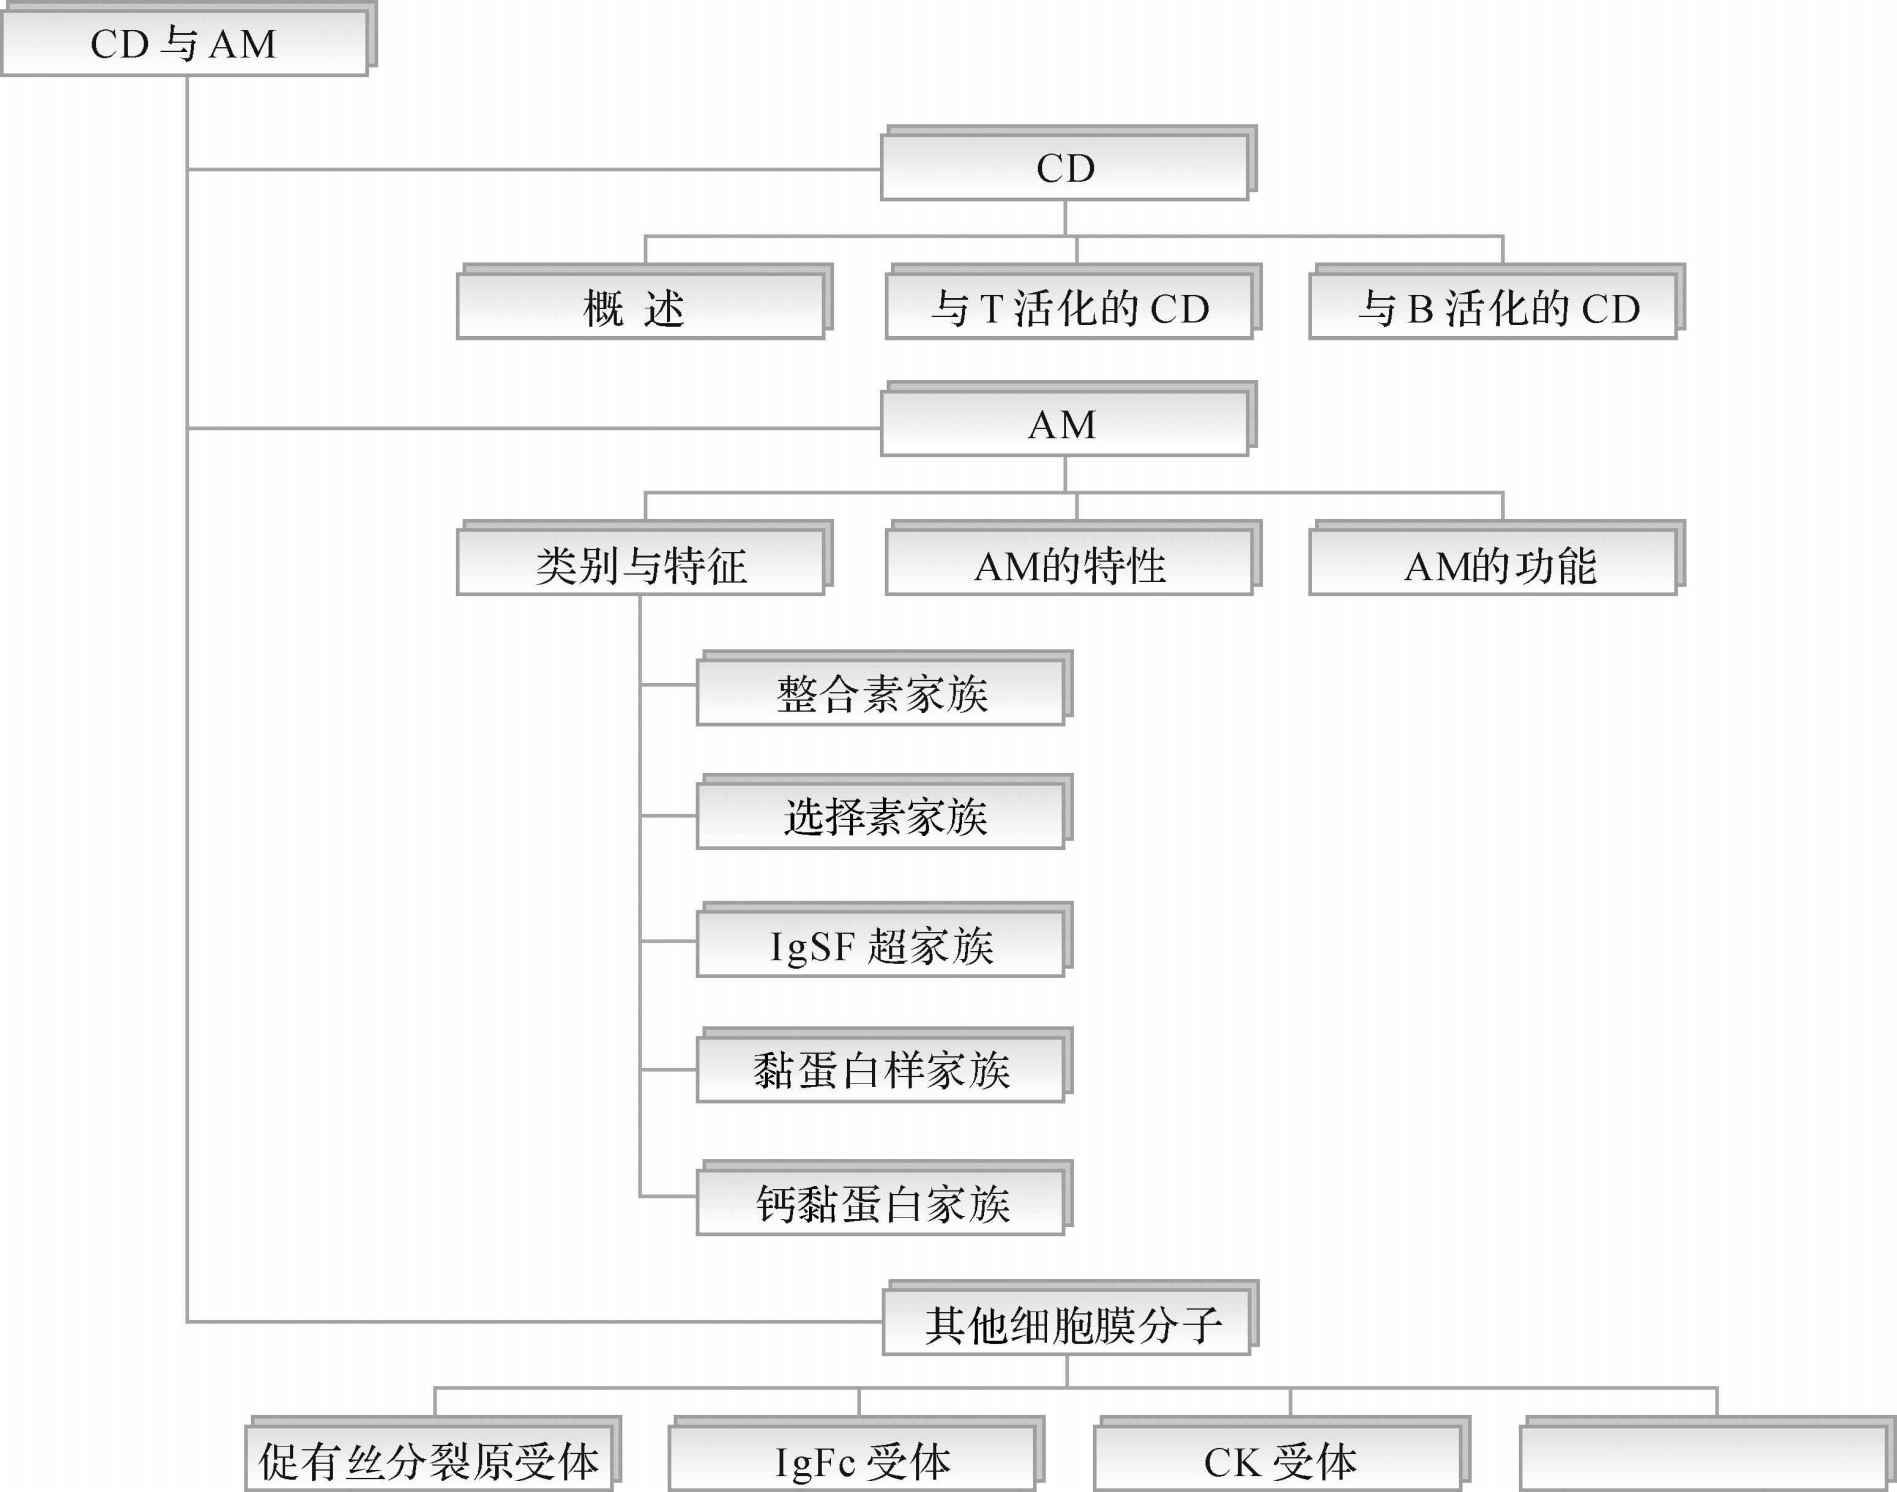
\includegraphics[width=.6\textwidth]{./images/Image00110.jpg}
\end{center}
\noindent\textbf{【课前思考】}

如同一个人体表有许多结构,起到不同的作用,参与免疫应答的免疫细胞膜表面也有许多特殊的结构,其到底有哪些分子结构?各有哪些作用?如何介导、参与细胞免疫应答、体液免疫应答?其他种类的免疫细胞膜分子还有哪些?

\noindent\textbf{【本章重点】}

1.白细胞分化抗原和黏附分子的概念、种类与作用;

2.参与T、B淋巴细胞分化的CD分子。

\noindent\textbf{【教学目标】}

1.掌握白细胞分化抗原和黏附分子的概念、种类与作用;

2.熟悉参与T、B淋巴细胞分化的CD分子。
\end{framed}

机体免疫系统是由中枢淋巴器官、外周淋巴器官、免疫细胞和免疫分子所组成。免疫应答过程有赖于免疫系统中细胞间的相互作用,包括细胞间直接接触和通过释放细胞因子或其他介质的相互作用。免疫细胞间或细胞与介质间相互识别的物质基础是免疫细胞膜分子,包括细胞表面的多种抗原、受体和其他分子。细胞膜分子通常也称为细胞表面标记(cell
surface
marker)。免疫细胞膜分子的种类相当繁多,主要有T细胞受体、B细胞识别抗原的膜免疫球蛋白、主要组织相容性复合体抗原、白细胞分化抗原、黏附分子、结合促分裂素的分子、细胞因子受体、免疫球蛋白Fc段受体以及其他受体和分子,不仅参与识别、捕捉抗原、免疫细胞与抗原、免疫分子间的相互作用,还能介导免疫细胞间、免疫细胞与基质间的黏附作用,在免疫应答的识别、活化及效应阶段均发挥重要作用。免疫细胞膜分子的研究有助于在分子水平认识免疫应答的本质,对疾病的诊断、预防、治疗和机制探讨具有重要意义。

\section{白细胞分化抗原}


\subsection{概述}

白细胞分化抗原(leukocyte differentiation
antigen,LDA)是白细胞(还包括血小板、血管内皮细胞等)在分化成熟为不同谱系(lin-eage)和分化不同阶段以及活化过程中,出现或消失的细胞表面标记。它们大都是穿膜的蛋白或糖蛋白,含胞膜外区、穿膜区和胞浆区;有些白细胞分化抗原是以糖基磷脂酰肌醇(glyco-sylphosphatidylinositol,GPI)连接方式“锚”在细胞膜上,少数白细胞分化抗原是碳水化合物半抗原。

白细胞分化抗原种类繁多,分布广泛,除表达于白细胞之外,还广泛分布于不同分化阶段的红细胞系、巨核细胞/血小板谱系和非造血细胞(如血管内皮细胞、成纤维细胞、上皮细胞、神经内分泌细胞等)表面。

白细胞分化抗原参与机体重要的生理和病理过程:(1)免疫应答过程中免疫细胞的相互识别,免疫细胞抗原识别、活化、增殖和分化,免疫效应功能的发挥;(2)造血细胞的分化和造血过程的调控;(3)炎症发生;(4)细胞的迁移如肿瘤细胞的转移等。本章仅介绍参与免疫细胞识别、信号转导以及活化与效应的CD分子。

早期各实验室多借助自制的特异性抗体对白细胞分化抗原进行分析和鉴定,故同一分化抗原可能有不同命名。20世纪80年代初以来,由于单克隆抗体,分子克隆、基因转染细胞系等技术在白细胞分化抗原研究中得到广泛深入的应用,有关白细胞分化抗原的研究和应用进展相当迅速。在世界卫生组织(WHO)和国际免疫学会联合会(IUIS)的组织下,自1982年至1993年已先后举行了五次有关人类白细胞分化抗原的国际协作组会议(International
workshop on human leukocyte differentiation
antigens),并应用以单克隆抗体鉴定为主的聚类分析法,将识别同一分化抗原的来自不同实验室的单克隆抗体归为一个分化群,简称CD(cluster
of
differentiation),以CD代替以往的命名。迄今,人CD的序号已从CD1命名至CD339。在许多场合下,抗体及其识别的相应抗原都用同一个CD序号。


\subsection{参与T细胞抗原识别与活化的CD分子}

T细胞是一类重要的免疫活性细胞,除直接介导细胞免疫功能外,对机体免疫应答的调节起关键作用。T淋巴细胞本身的识别活化及效应功能的发挥,不仅与外来抗原、丝裂原和多种细胞因子密切相关,而且有赖于T细胞相互之间、T细胞与抗原递呈细胞(APC)之间以及T细胞与靶细胞之间的直接接触。T淋巴细胞识别抗原的受体是T细胞受体(T
cell
receptor,TCR)与CD3所组成的复合物(TCR-CD3)。在识别过程中还有赖于抗原非特异性的其他细胞表面分子的辅助,这些辅助分子(accessory
molecules)主要包括CD4、CD8、CD2、CD28、CD40L、CD58、CD80、CD86和CD152等(图\ref{fig8-1})。

\begin{figure}[!htbp]
 \centering
 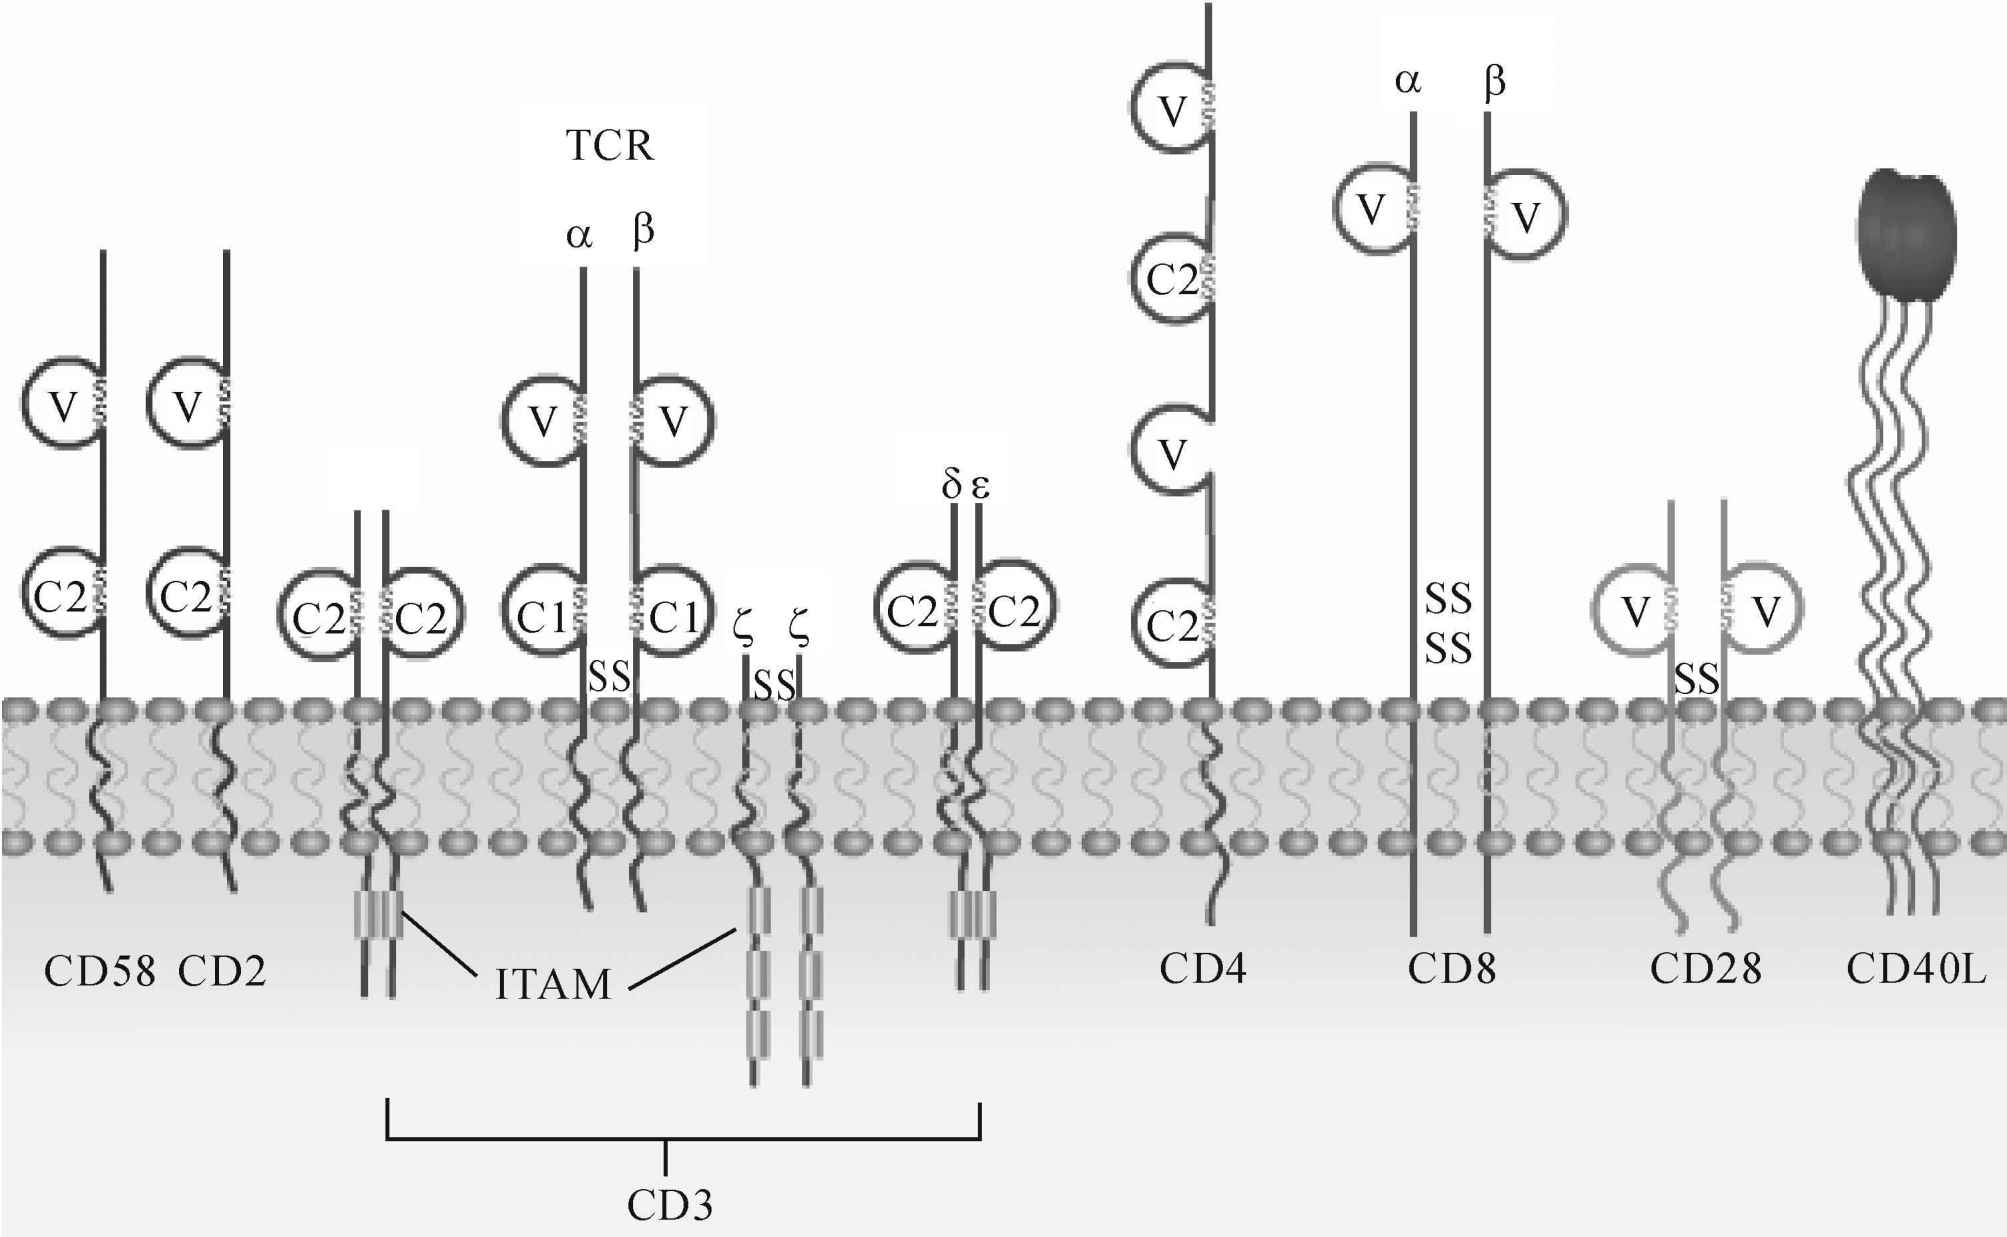
\includegraphics{./images/Image00111.jpg}
 \captionsetup{justification=centering}
 \caption{参与T细胞抗原识别与活化的CD分子}
 \label{fig8-1}
  \end{figure} 

1.CD3

CD3由γ、δ、ε、ζ、η五种肽链组成,通过盐桥与T细胞受体TCR形成TCR-CD3复合体,分布于所有成熟T细胞和部分胸腺细胞表面。

CD3的主要功能是转导TCR特异性识别抗原所产生的活化信号,促进T细胞活化。CD3分子胞浆区含免疫受体酪氨酸活化基序(immunoreceptor
tyrosine-based activation
motif,ITAM),TCR识别或结合由MHC分子递呈的抗原肽后,导致ITAM所含酪氨酸磷酸化,通过活化相关激酶,将识别信号转入T细胞内(图\ref{fig8-2})。CD3是参与TCR信号转导的关键分子,CD3肽链缺陷或缺失,可导致T细胞活化缺陷。

\begin{figure}[!htbp]
 \centering
 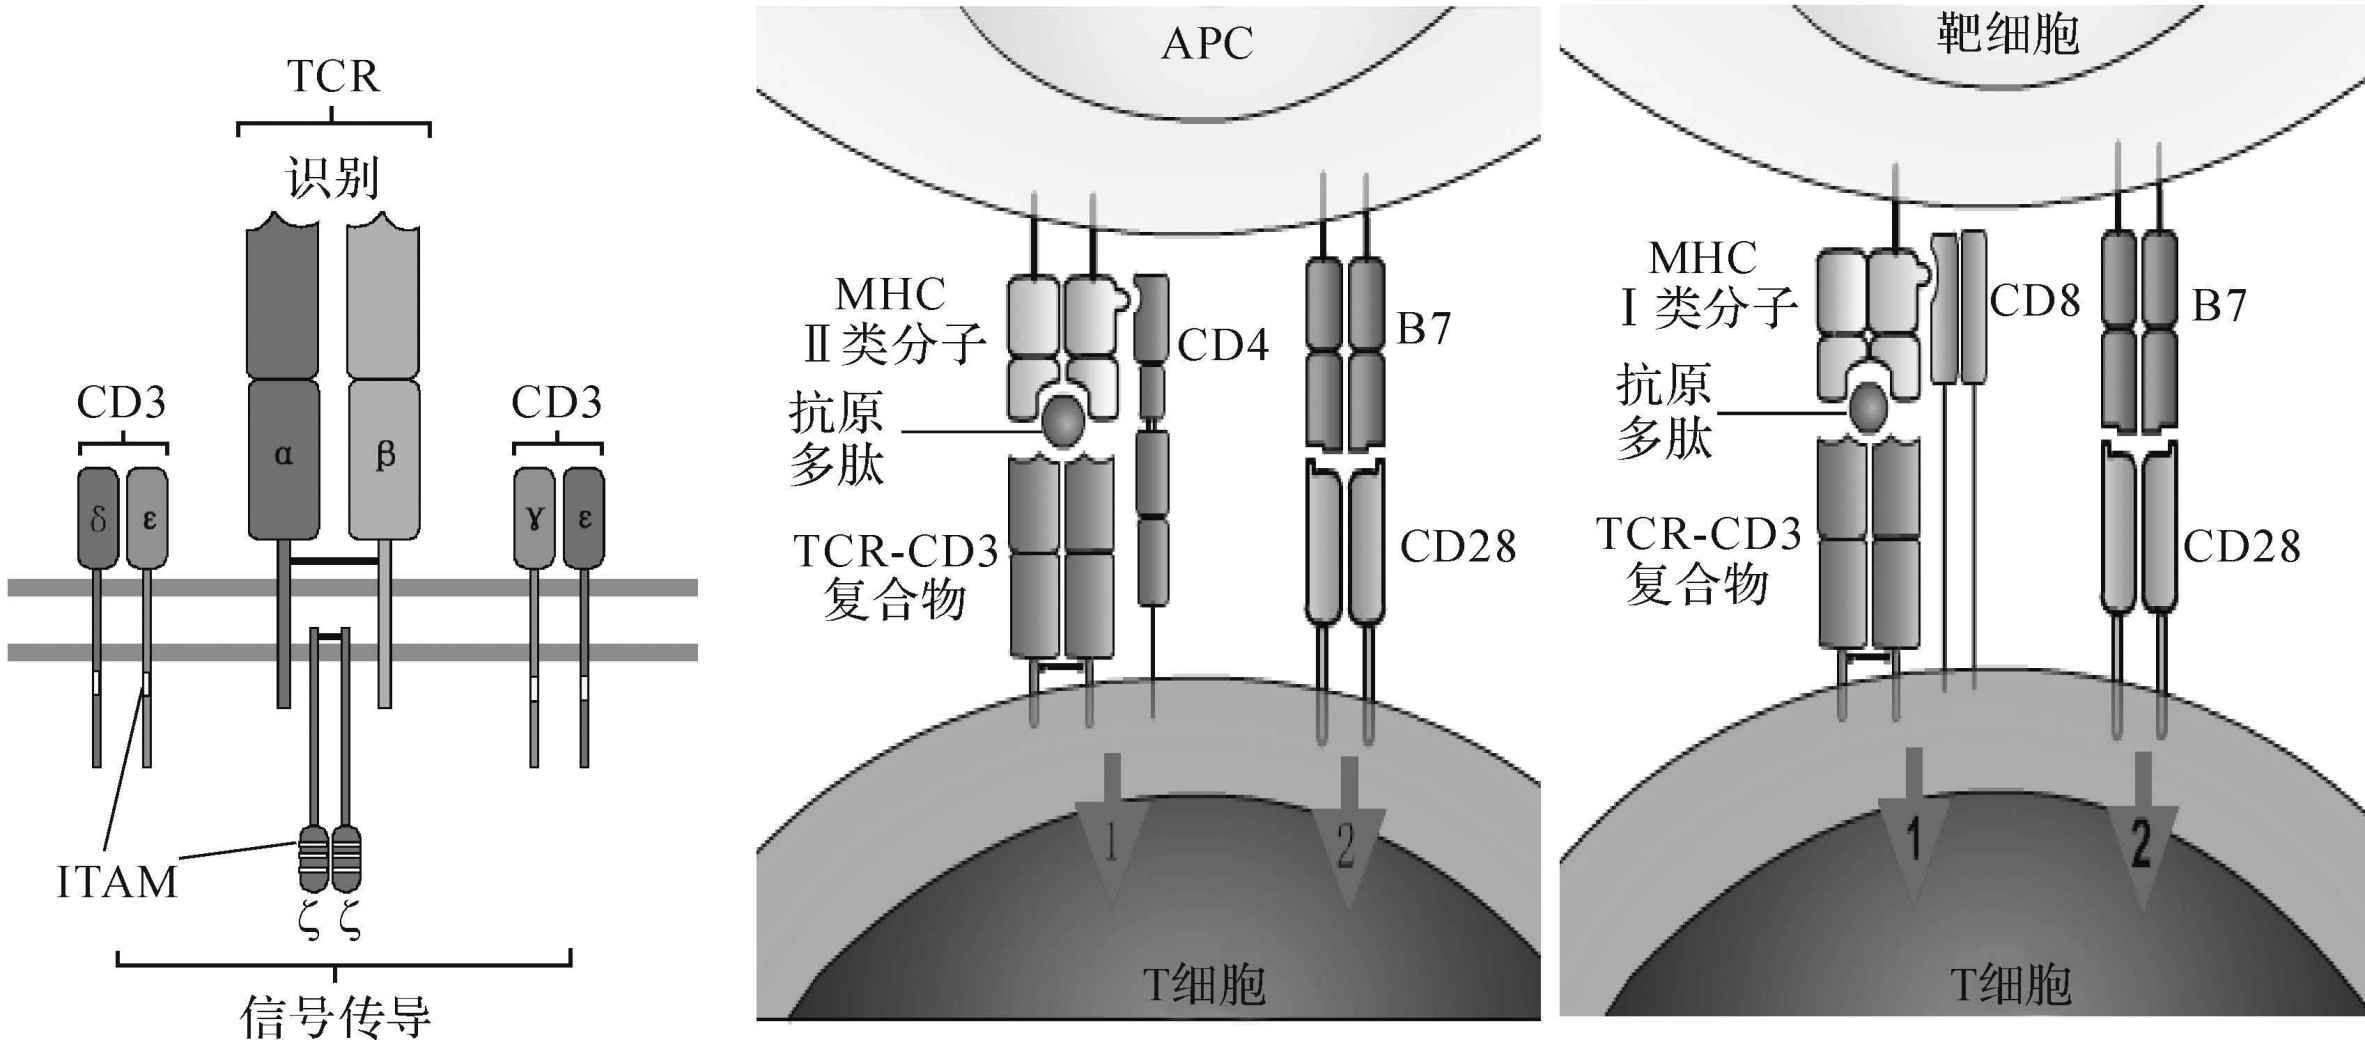
\includegraphics{./images/Image00112.jpg}
 \captionsetup{justification=centering}
 \caption{活化信号}
 \label{fig8-2}
  \end{figure} 

2.CD4

CD4为单链跨膜糖蛋白,属免疫球蛋白超家族(IgSF)成员,分布于胸腺细胞和成熟TH细胞,也存在于巨噬细胞、脑细胞。在外周血和淋巴器官中,CD4\textsuperscript{+}
T细胞主要为辅助性T细胞(helper T
cell,Th)。功能:(1)作为TH与APC之间的黏附分子,CD4/MHC-II类。(2)信号转导作用:细胞内传导。CD4分子也是人类免疫缺陷病毒(HIV)受体。

3.CD8

CD8也属IgSF成员,分布于部分T细胞、胸腺细胞和NK细胞表面,通常作为判别T细胞的表面标志。功能:(1)介导细胞间黏附作用:CD8与MHC-I类结合,激活CTL。(2)信号传导:CD8-MHC-I
结合,启动T细胞免疫应答。

4.CD28与CD80(B7-1)/CD86(B7-2)

CD28分子乃借二硫键相连的同源二聚体,属IgSF成员。在外周血淋巴细胞中,几乎所有CD4\textsuperscript{+}
T细胞和50%CD8\textsuperscript{+}
T细胞表达CD28。此外,浆细胞和部分活化B细胞也可表达CD28。一般而言,活化T细胞CD28表达水平升高。

CD28分子胞浆区可与多种信号分子相连,能转导T细胞活化的共刺激信号。CD28的配体是表达于B细胞和APC表面的B7家族分子,包括CD80(B7-1)和CD86(B7-2)。CD28/B7-1、B7-2是一组最重要的共刺激分子,它们之间结合提供T细胞活化所必需的共刺激信号,即第二信号。

5.CD2 /CD58

\begin{figure}[!htbp]
 \centering
 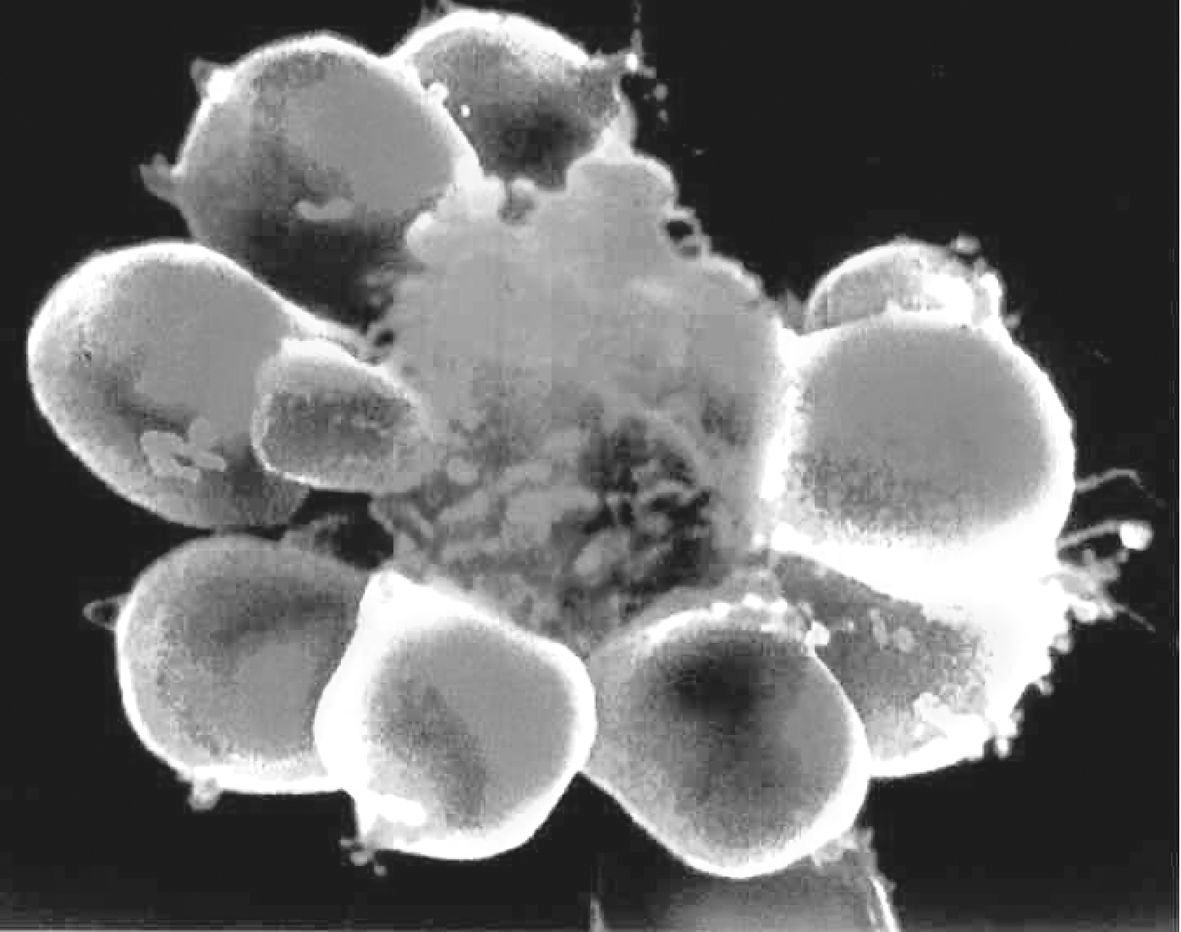
\includegraphics[width=.6\textwidth]{./images/Image00113.jpg}
 \captionsetup{justification=centering}
 \caption{E花环}
 \label{fig8-3}
  \end{figure} 

CD2 又称淋巴细胞功能相关抗原2(lymphocyte function associated antigen
2,LFA-2)或绵羊红细胞受体(sheep red cell
receptor,SRBC),表达于T细胞、胸腺细胞和NK细胞等。人CD2的配基是CD58(LFA-3)分子,二者结构相似,且均属IgSF成员。

CD58分布较广,包括多种血细胞和某些非造血细胞。CD2与CD58结合能增强T细胞与APC或靶细胞间黏附,促进T细胞对抗原识别和CD2所介导的信号转导。此外,人T细胞还能通过CD2与SRBC表面的CD58类似物结合形成花环,称为E花环(图\ref{fig8-3}),可用于体外检测和分离T细胞。


\subsection{参与B细胞识别Ag与活化的CD分子}

B细胞抗原受体(BCR、SmIg)、CD19/CD21/CD81、CD40与CD40L等(图\ref{fig8-4})。

\begin{figure}[!htbp]
 \centering
 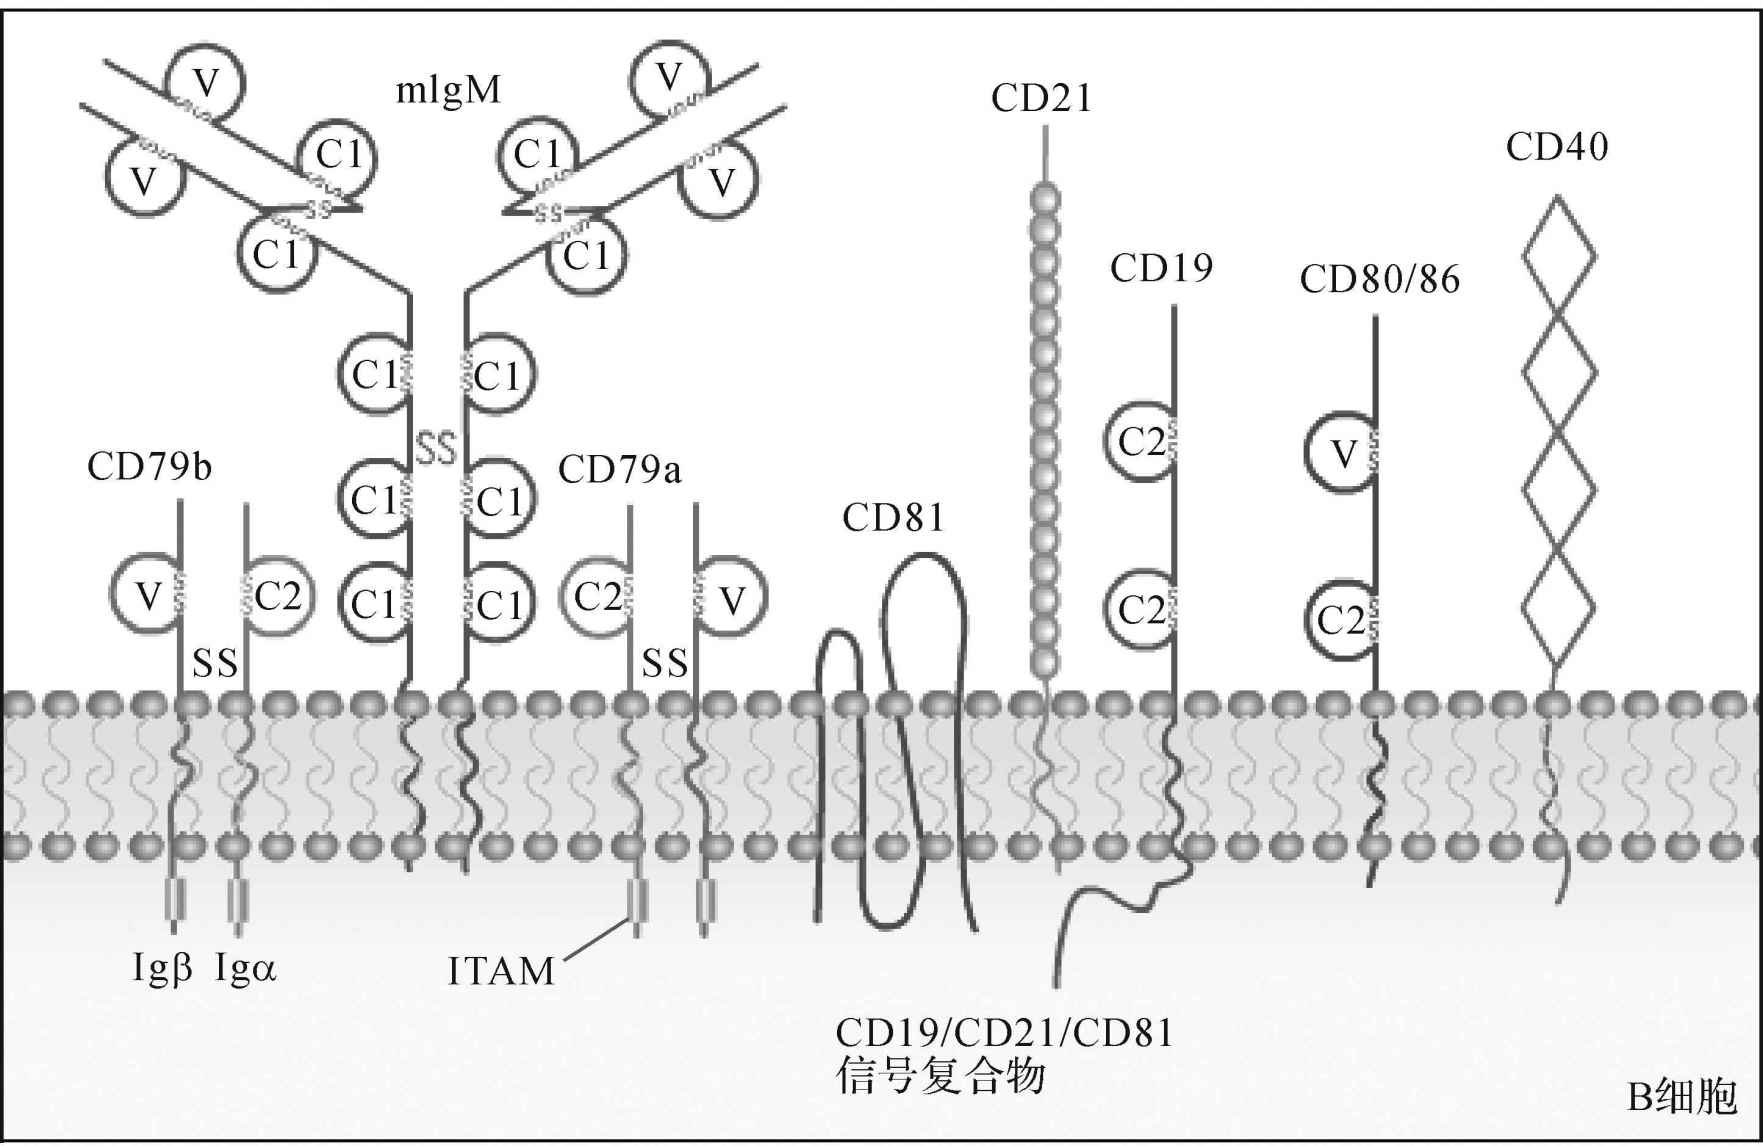
\includegraphics{./images/Image00114.jpg}
 \captionsetup{justification=centering}
 \caption{参与B细胞抗原识别与活化的CD分子}
 \label{fig8-4}
  \end{figure} 

1.B细胞抗原受体(BCR、SmIg)

B细胞抗原受体是B细胞特异性应答的关键分子(图\ref{fig8-5})。BCR特异性识别并结合抗原。BCR也有两种辅助成分,即Ig-I(CD79a)和Ig-I(CD79b)。在人类B细胞中,与mIgM相关的Igα和Igβ分别为47kDa和37kDa糖蛋白,属于免疫球蛋白超家族成员,通过非共价键成为BCR-Igα/Igβ复合体。Igα和Igβ胞膜外区氨基端处均有一个Ig样结构域。Igα和Igβ均可作为蛋白酪氨酸激酶的底物,可能与BCR信号转导有关,因为mIgM和mIgD胞浆区只有3个氨基酸(KVK),不可能单独把胞膜外的刺激信号传递到细胞内。

\begin{figure}[!htbp]
 \centering
 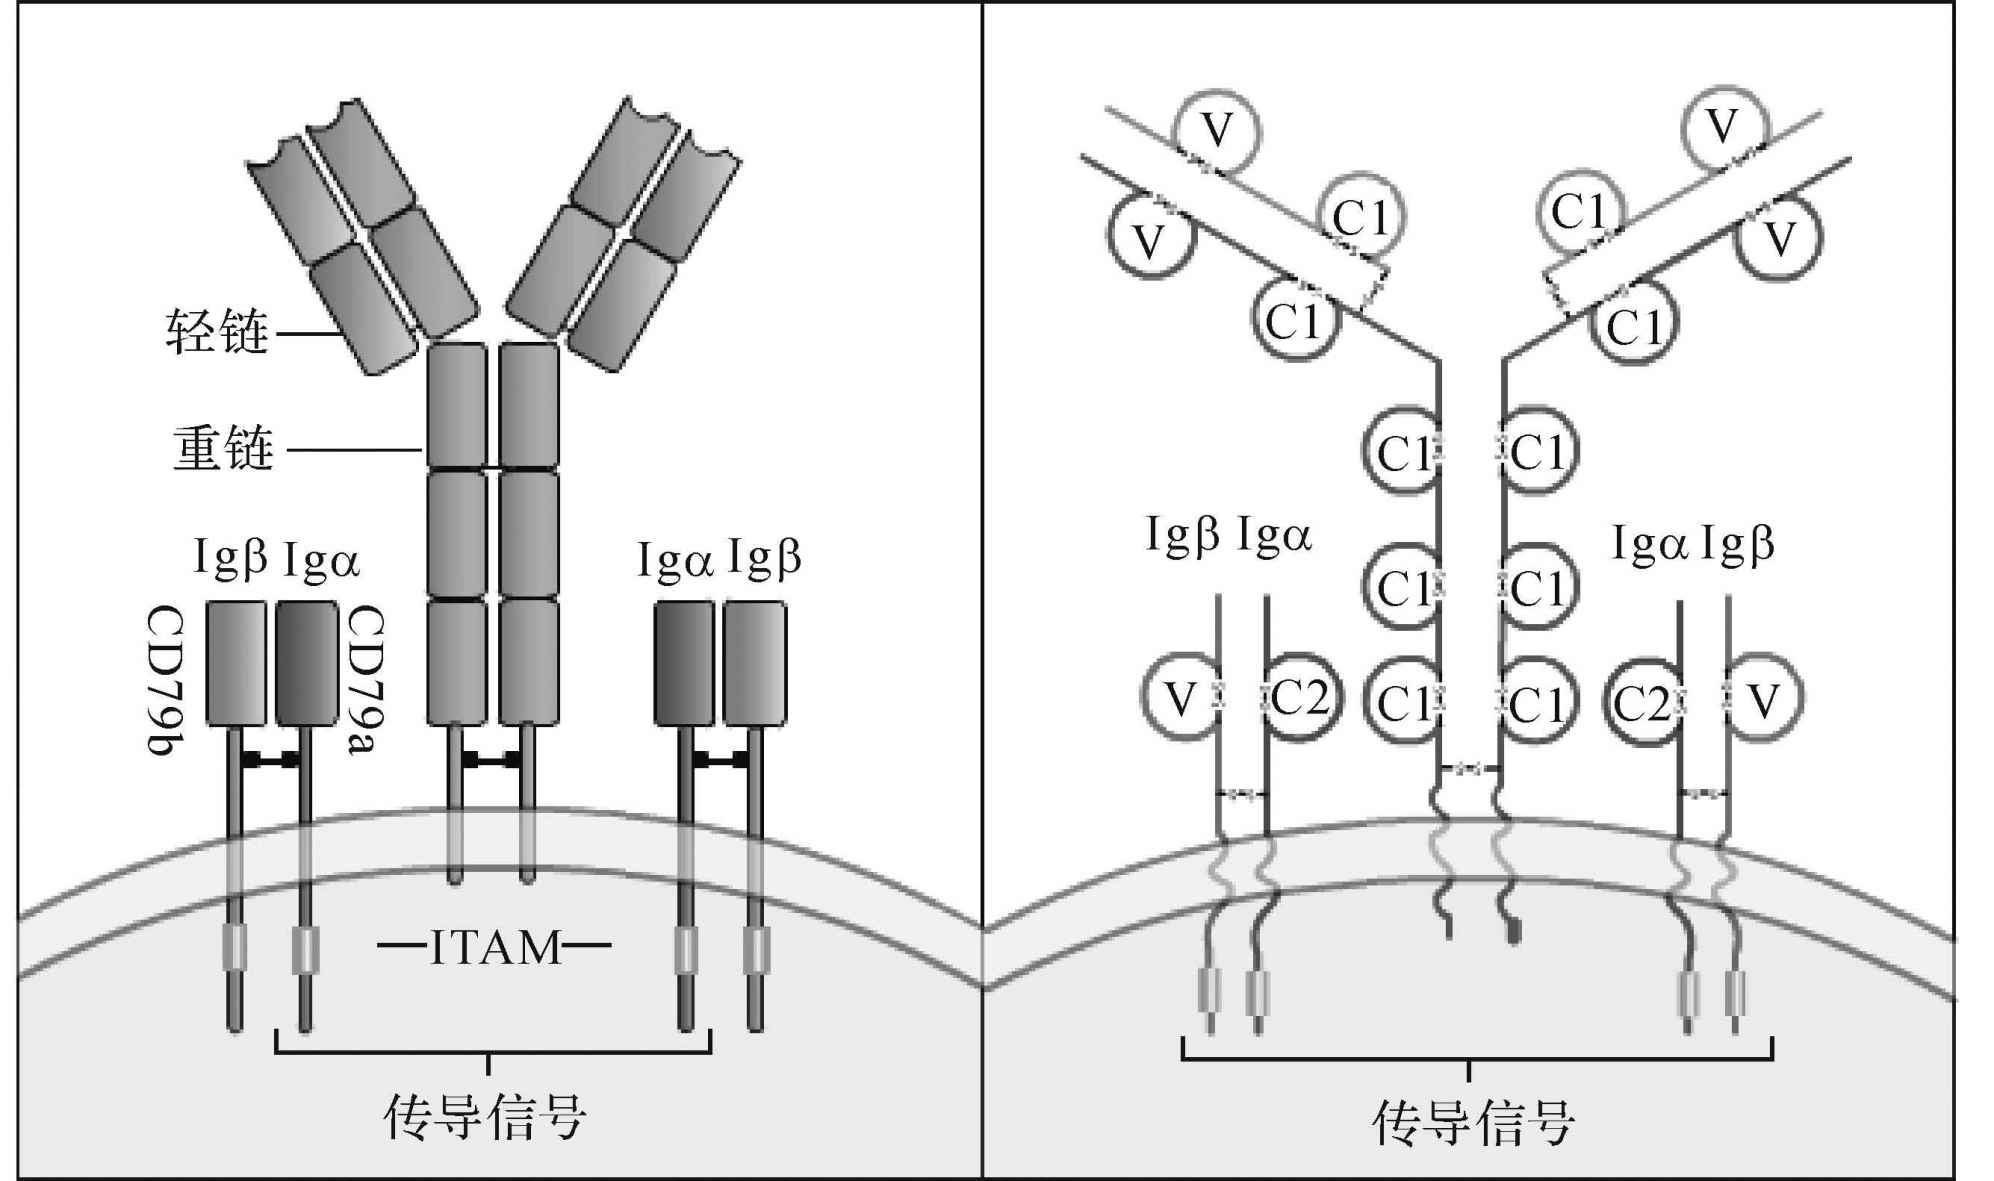
\includegraphics{./images/Image00115.jpg}
 \captionsetup{justification=centering}
 \caption{B细胞抗原受体结构示意图}
 \label{fig8-5}
  \end{figure} 

2.CD19/CD21/CD81

CD19、CD21、CD81构成的复合物是B细胞活化的共受体,通过CD19分子胞浆区与多种激酶的结合,能加强跨膜信号转导,促进B细胞活化。CD19/CD21/CD81信号复合物可调节BCR活化的阈值,其中CD21(CR2)借助补体C3片段而介导CD19与BCR交联,从而促进B细胞活化,这对B细胞初次应答尤为重要(图\ref{fig8-6})。

\begin{figure}[!htbp]
 \centering
 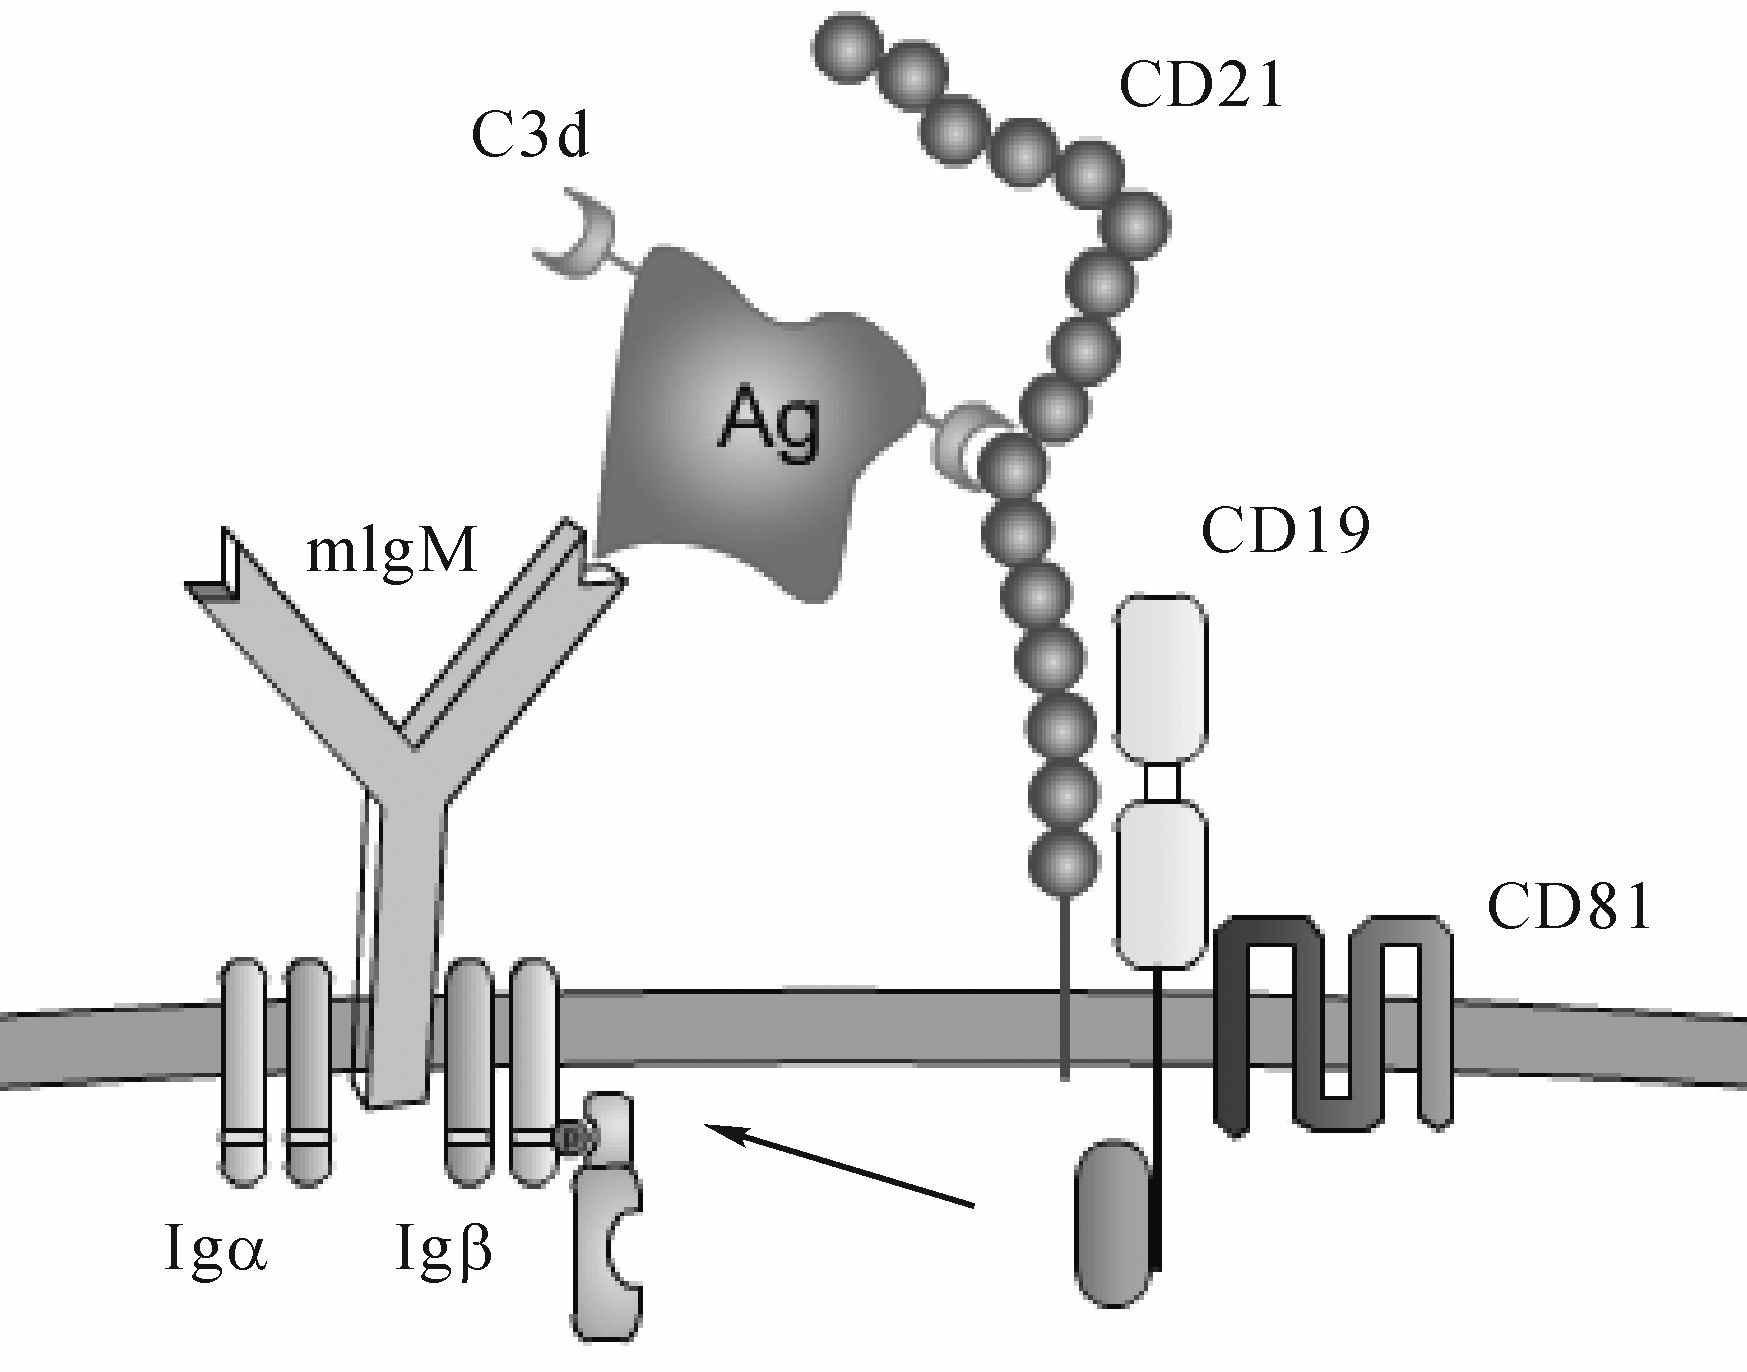
\includegraphics{./images/Image00116.jpg}
 \captionsetup{justification=centering}
 \caption{B细胞信号复合物示意图}
 \label{fig8-6}
  \end{figure} 

CD19分布于除浆细胞外不同发育阶段的B细胞表面,是鉴定B细胞的重要标志之一。CD21是CR2、C3dR、EB病毒的受体,仅表达于静止的成熟的B细胞表面,B细胞一旦活化即消失,是B细胞的重要标志。CD81广泛分布于B细胞、T细胞、巨噬细胞、树突状细胞、NK细胞和嗜酸粒细胞表面。CD81是丙型肝炎病毒(HCV)受体,可能参与HBV感染。

3.CD40与CD40L

CD40分子属肿瘤坏死因子超家族,主要分布于B细胞、树突状细胞以及某些上皮细胞、内皮细胞、成纤维细胞和活化的单核细胞表面。

CD40L即CD40配体,属IgSF家族成员。人CD40L主要表达在活化CD4\textsuperscript{+}
T细胞、部分CD8\textsuperscript{+}
T细胞和γδT细胞表面。CD40L与B细胞表面CD40结合是B细胞再次免疫应答和生发中心形成的必要条件。T细胞表面CD40L与B细胞表面CD40结合,能提供B细胞活化所需的共刺激信号,这是B细胞对TD抗原产生应答的重要条件。CD40L也能激活单核/巨噬细胞。CD40与CD40L的相互作用还参与淋巴细胞发育的阴性选择过程和外周免疫耐受的形成。此外,CD40L还表达于活化的嗜碱粒细胞、肥大细胞、NK细胞、单核细胞以及活化B细胞表面。

\section{黏附分子}

黏附分子(adhesion
molecule,AM)是一类介导细胞与细胞间或细胞与细胞外基质(extracell
matrix,ECM)间相互接触和结合的分子,多为跨膜糖蛋白。黏附分子广泛分布于几乎所有细胞表面,某些情况下也可从细胞表面脱落至体液中,成为可溶性黏附分子(soluble
adhesion
molecule)。黏附分子以配体-受体结合的形式发挥作用,参与细胞识别、信号转导以及细胞活化、增殖、分化与移动等,是免疫应答、炎症反应、凝血、创伤愈合以及肿瘤转移等一系列重要生理与病理过程的分子基础。

黏附分子与CD分子是根据不同角度命名的膜分子:黏附分子乃以黏附功能归类;CD分子是借助单克隆抗体鉴定、归类而命名。一大类CD分子具有黏附作用,大部分黏附分子也属CD分子。


\subsection{黏附分子的类别及其特征}

根据黏附分子的结构特点可将其分为整合素、选择素、黏蛋白样、免疫球蛋白超家族及钙黏蛋白5个家族,此外还有一些尚未归类的黏附分子。

(一)整合素家族(integrin family)

整合素乃因其主要介导细胞与细胞外基质(ECM)的黏附,使细胞附着以形成整体而得名(图\ref{fig8-7})。整合素参与细胞活化、增殖、分化、吞噬与炎症形成等多种功能。

\begin{figure}[!htbp]
 \centering
 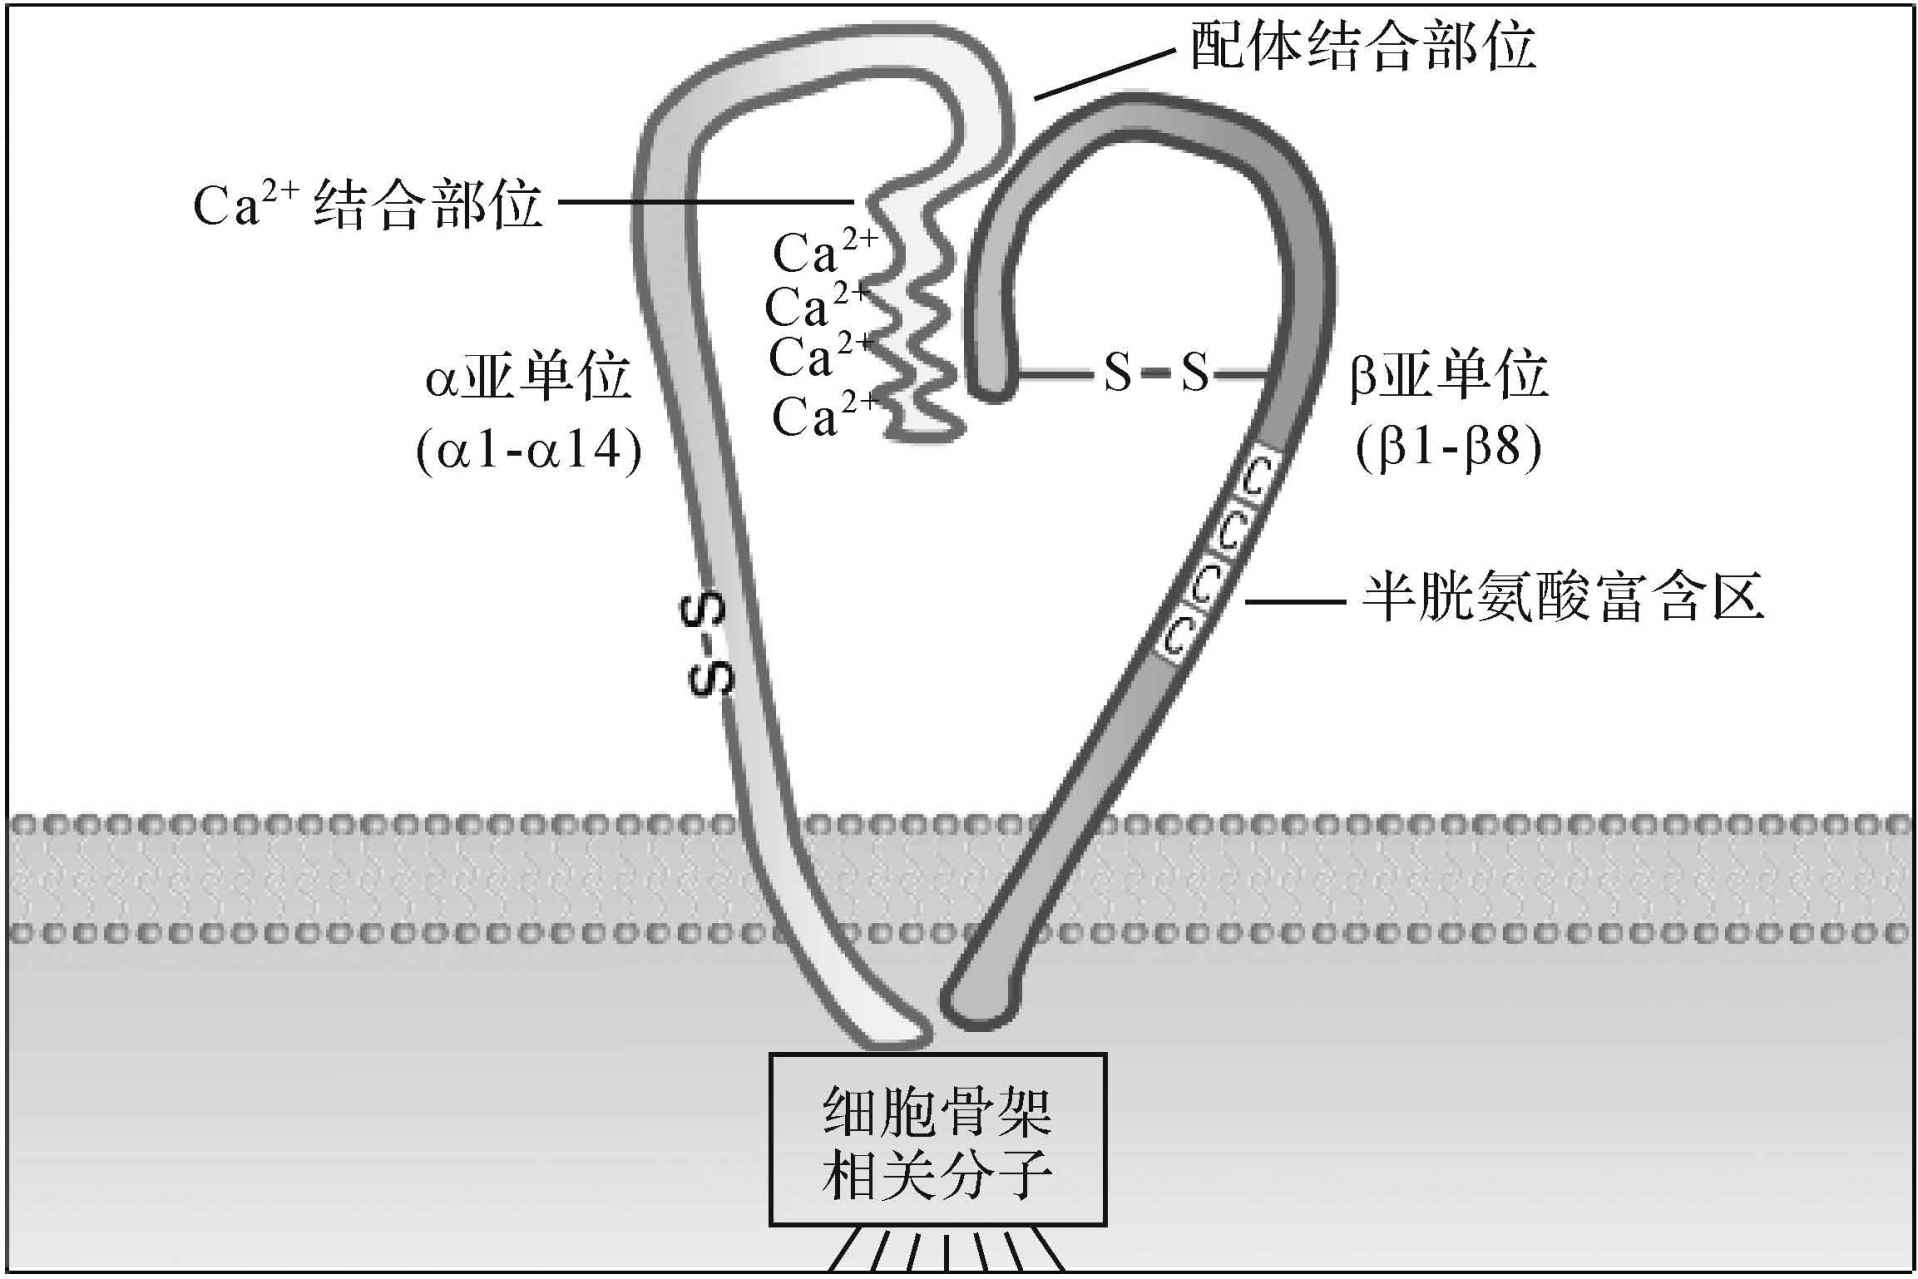
\includegraphics{./images/Image00117.jpg}
 \captionsetup{justification=centering}
 \caption{典型整合素分子结构示意图}
 \label{fig8-7}
  \end{figure} 

整合素家族成员均为α、β两条多肽链(或亚单位)组成的异源二聚体。目前已知整合素家族中至少有14种α链亚单位和8种β链亚单位。迄今已发现20余个整合素家族成员,按β链亚单位的不同,可将其分为β1~β8共8个组。同一组成员的β链均相同,而α链各异。多数α链亚单位仅能与一种β链亚单位结合,而多数β链亚单位则可结合数种不同α链亚单位。

整合素家族是介导细胞与ECM相互黏附的重要分子,其配体主要是ECM蛋白(如纤连蛋白、血纤蛋白原、玻连蛋白等)。某些整合素配体是细胞表面分子,可介导细胞间相互作用。

(二)选择素家族(selectin family)

参与炎症发生、淋巴细胞归巢、凝血以及肿瘤转移等,包括L-选择素(CD62L)、P-选择素(CD62P)和E-选择素(CD62E)3个成员,L、P、E分别代表最初发现此3种选择素的白细胞、血小板和血管内皮细胞(图\ref{fig8-8})。选择素分子的配体是一些寡糖基团,主要是唾液酸化的路易斯寡糖(sialyl
Lweis,sLex
或CD15s)或具有类似结构的分子。此类配体主要分布于白细胞、血管内皮细胞及某些肿瘤细胞表面。

\begin{figure}[!htbp]
 \centering
 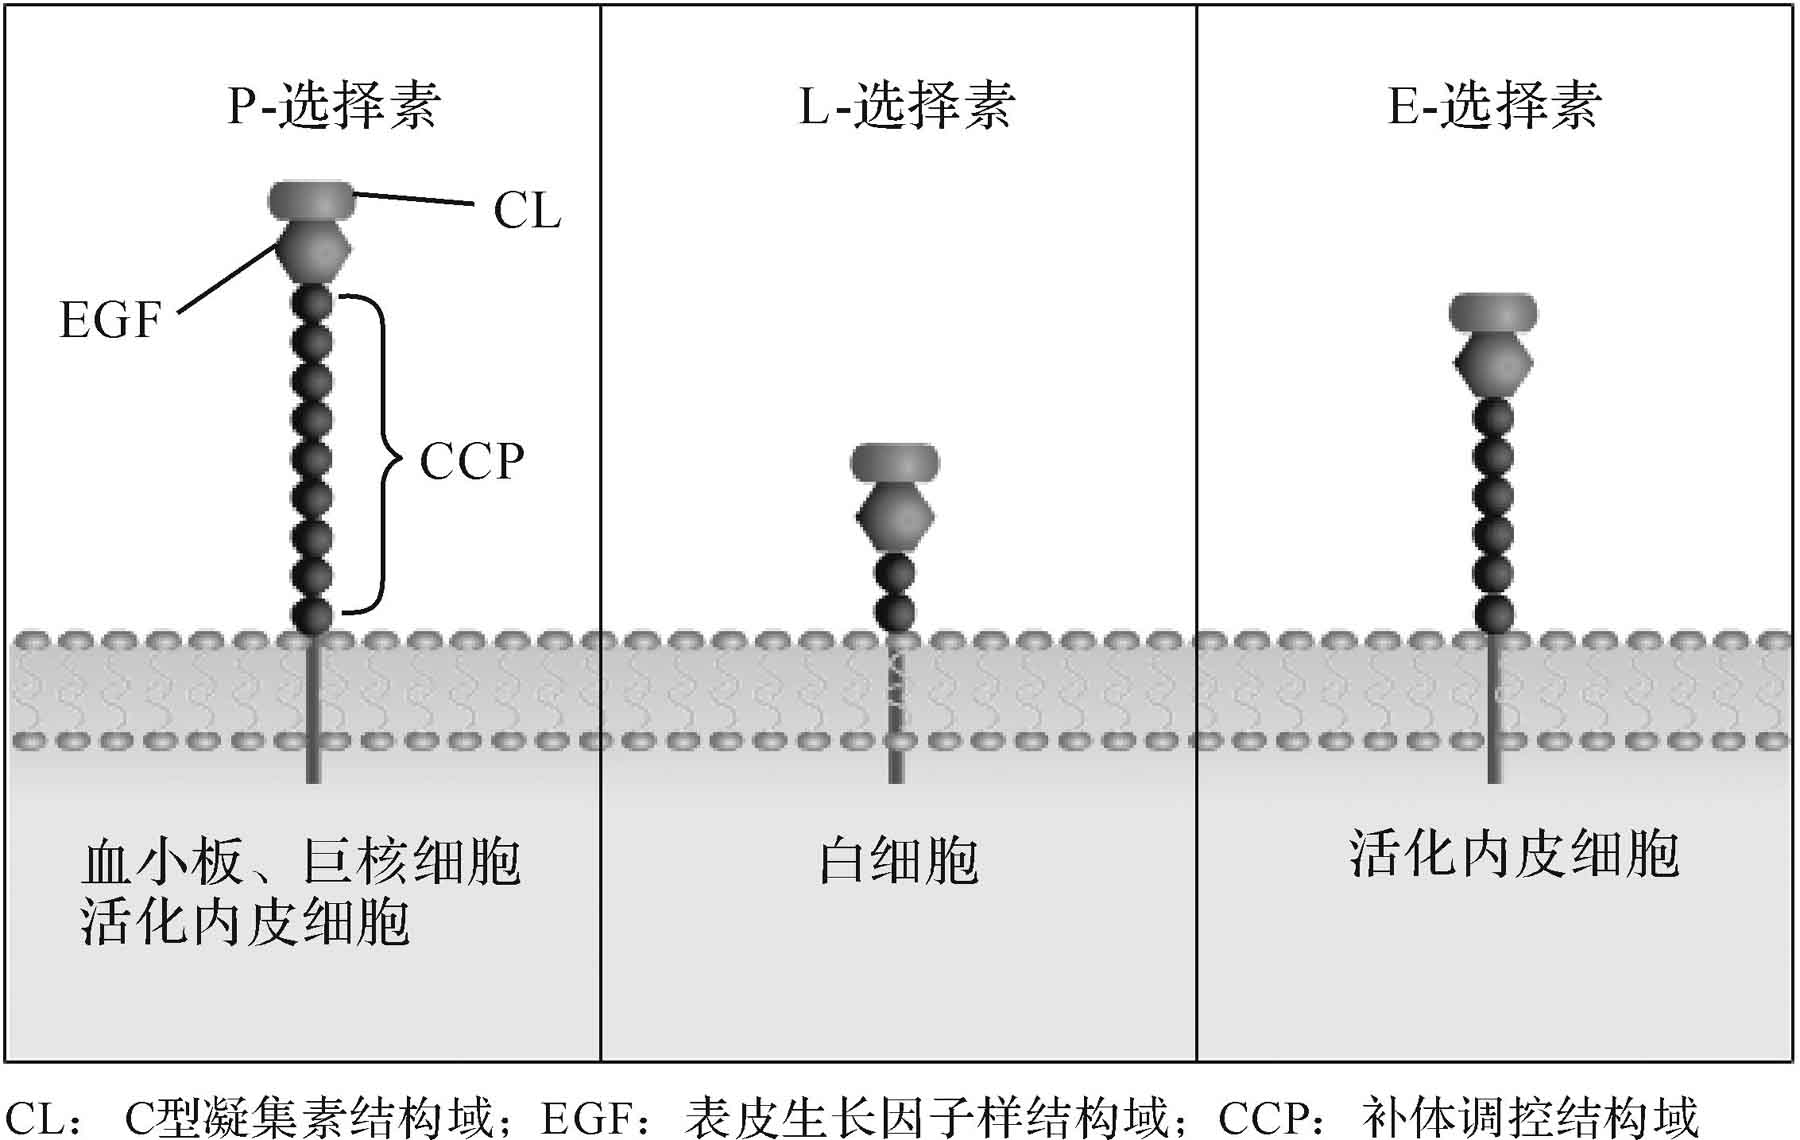
\includegraphics{./images/Image00118.jpg}
 \captionsetup{justification=centering}
 \caption{选择素家族黏附分子}
 \label{fig8-8}
  \end{figure} 

(三)免疫球蛋白超家族(immunoglobulin superfamily,IgSF)

这是一类具有类似于IgV区或C区折叠结构、氨基酸组成也与Ig有一定同源性的分子。IgSF成员极多,包括抗原特异性受体(如TCR
与BCR)、非抗原特异性受体及其配体(如CD2与LFA-3)、IgFc受体、某些黏附分子及MHC-Ⅰ、Ⅱ类分子等(表\ref{tab8-1})。属于IgSF成员的黏附分子,其识别的配体多为IgSF分子或整合素分子,主要介导T细胞-APC/靶细胞、T细胞-B细胞间的相互识别与作用。

\begin{longtable}[]{@{}lll@{}}
    \caption{IgSF黏附分子的种类、分布和配体}
    \label{tab8-1}\\
\toprule
IgSF 黏附分子 & 分  布 & 配  体\tabularnewline
\midrule
\endhead
L FA‐2(CD2) & T 细胞、胸腺细胞、NK 细胞 & L FA‐3(IgSF
)\tabularnewline
L FA‐3(CD58) & 广泛 & L FA‐2(IgSF )\tabularnewline
ICAM‐1(CD54) & 广泛 & L FA‐1(整合素家族)\tabularnewline
ICAM‐2(CD102) & 内皮细胞、T 细胞、B 细胞、髓样细胞 & L
FA‐1(整合素家族)\tabularnewline
ICAM‐3(CD50) & 白细胞 & L FA‐1(整合素家族)\tabularnewline
CD4 & 辅助性T细胞亚群 & MHC‐II(IgSF)\tabularnewline
CD8 & 杀伤性T细胞亚群 & MHC‐I(IgSF)\tabularnewline
MHC‐I & 广泛 & CD8(IgSF )\tabularnewline
MHC‐II & B 细胞、活化T 细胞、活化内皮细胞、巨噬细胞、树突状细胞 &
CD4(IgSF )\tabularnewline
CD28 & T细胞、活化B细胞 & B7‐1(IgSF)\tabularnewline
B7‐1(CD80) & 活化B 细胞、活化单核细胞 & CD28(IgSF )\tabularnewline
NCAM‐1(CD56) & NK 细胞、神经元 & NCAM‐1(IgSF )\tabularnewline
VCAM‐1(CD106) & 内皮细胞、树突状细胞、巨噬细胞 & VL
A‐4(整合素家族)\tabularnewline
PECAM‐1(CD31) & 白细胞、血小板、内皮细胞 & PECAM‐1(IgSF
)\tabularnewline
\bottomrule
\end{longtable}

(四)黏蛋白样家族(mucin-like family)

这是一组富含丝氨酸和苏氨酸的糖蛋白,为新归类的一类黏附分子。该家族包括CD34、糖酰化依赖的细胞黏附分子-1(glycosylation-dependent
cell adhesion molecule-1,GlyCAM-1)和P选择素糖蛋白配体(P-selectin
glycoprotein
ligand-1,PSGL-1)3个成员。此类黏附分子膜外区均可为选择素提供唾液酸化的糖基配位,故可与选择素结合。

CD34是L-选择素的配体,主要分布于造血干细胞(HSC)、定向祖细胞、骨髓基质细胞和某些淋巴结的血管内皮细胞表面,参与早期造血的调控和淋巴细胞归巢。此外,部分急性非淋巴细胞白血病细胞、急性B细胞白血病细胞及血管来源的肿瘤细胞也表达CD34。

(五)钙黏蛋白家族(Ca\textsuperscript{2+} dependent adhesion molecule
family)

这是一类钙离子依赖的黏附分子家族。钙黏蛋白家族成员在体内有各自独特的组织分布,且可随细胞生长、发育状态不同而改变。钙黏蛋白为单链糖蛋白,多数钙黏蛋白膜外区结构相似,能介导相同分子的黏附,称同型黏附作用。

钙黏蛋白家族成员至少有20多个,其中与免疫学关系密切的主要是E-Cadherin、N-Cadherin和P-Cadherin三种,E、N、P分别表示上皮、神经和胎盘。钙黏蛋白在调节胚胎形态发育和实体组织形成与维持中具有重要作用。此外,肿瘤细胞钙黏蛋白表达改变与肿瘤细胞浸润和转移有关。

除上述五类黏附分子家族外,还有一些尚未归类的黏附分子,如外周淋巴结地址素(PNAd)、皮肤淋巴细胞相关抗原(CLA)、CD36和CD44等,它们分别具有介导炎症和淋巴细胞归巢等功能。


\subsection{黏附分子的特性}

1.受体与配体的结合是可逆性,也非高度特异性,同一黏附分子可与不同配体结合,与抗原---抗体结合不同。

2.同一种属不同个体的同类黏附分子基本相同,无多态性。

3.同一细胞表面可表达多种不同类型黏附分子。

4.黏附分子的作用往往通过多对受体-配体共同完成。

5.同一黏附分子,在不同细胞表面其功能不一。


\subsection{黏附分子的功能}

黏附分子参与机体多种重要的生理功能和病理过程,主要有免疫细胞识别中的辅助受体和辅助活化信号、炎症过程中白细胞与血管内皮细胞黏附和淋巴细胞归巢等。

(一)淋巴细胞活化的辅助信号分子

辅助受体和辅助活化信号是指免疫细胞在接受抗原刺激的同时,还必须有辅助的受体接受辅助活化信号才能被活化。辅助受体的种类很多,在不同的环境中发挥的作用也不相同,最为常见的提供辅助刺激信号的T细胞上黏附分子结合抗原递呈细胞(APC)上相应黏附分子有:CD4/MHC-Ⅱ类分子、CD8/MHC-Ⅰ类分子、CD28/CD80及CD86、CD2/CD58、LFA-1/ICAM-1等(图\ref{fig8-9})。T细胞识别APC细胞递呈的抗原后,如缺乏CD80(或CD86)提供的辅助刺激信号,则T细胞的应答处于无能状态。

\begin{figure}[!htbp]
 \centering
 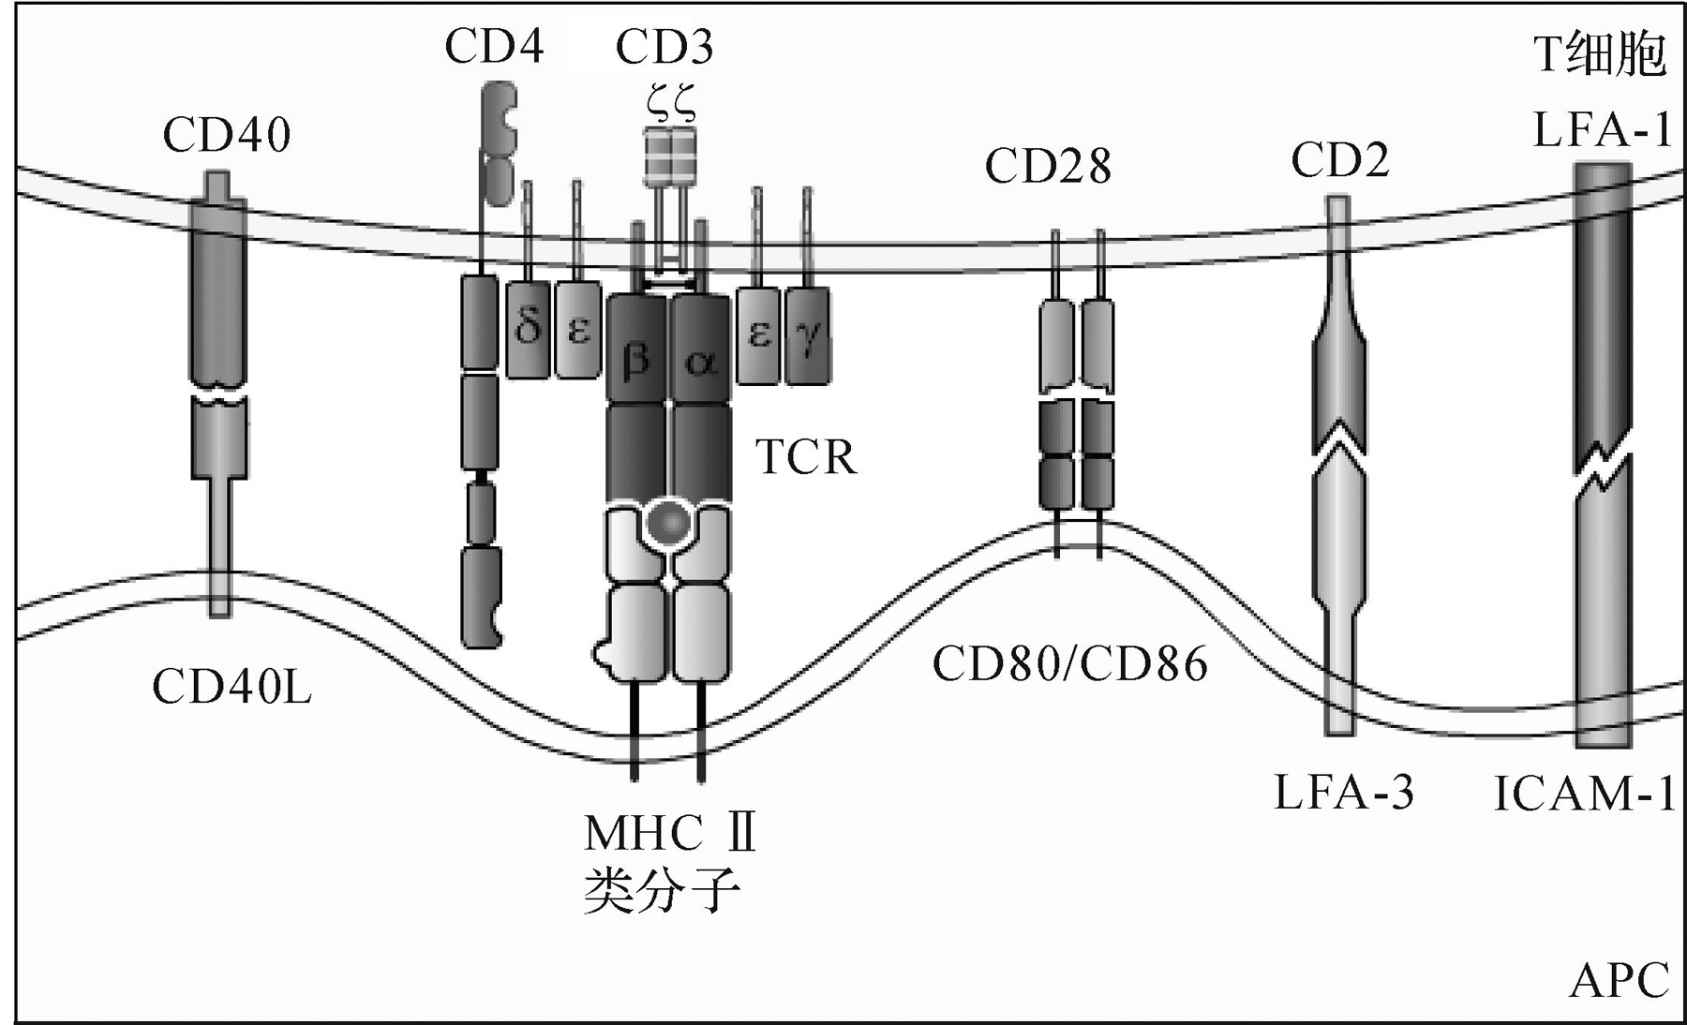
\includegraphics{./images/Image00119.jpg}
 \captionsetup{justification=centering}
 \caption{T细胞与APC间的主要黏附分子}
 \label{fig8-9}
  \end{figure} 

(二)介导白细胞与血管内皮细胞黏附

炎症过程的重要特征之一是白细胞与血管内皮细胞的黏附、穿越血管内皮细胞并向炎症部位渗出。该过程的重要分子基础是白细胞与血管内皮细胞间黏附分子的相互作用(图\ref{fig8-10})。不同白细胞的渗出过程或在渗出的不同阶段,其所涉及的黏附分子不尽相同。例如:炎症发生初期,中性粒细胞表面CD15s(SLex)可与血管内皮细胞表面E-选择素结合而黏附于管壁;随后,在血管内皮细胞表达的膜结合型IL-8诱导下,已黏附的中性粒细胞LFA-1和Mac-1等整合素分子表达上调,同内皮细胞表面由促炎因子诱生的ICAM-1相互结合,对中性粒细胞与内皮细胞紧密黏附和穿越血管壁到炎症部位均发挥关键作用。淋巴细胞的黏附、渗出过程与中性粒细胞相似,但参与的黏附分子有所不同。

\begin{figure}[!htbp]
 \centering
 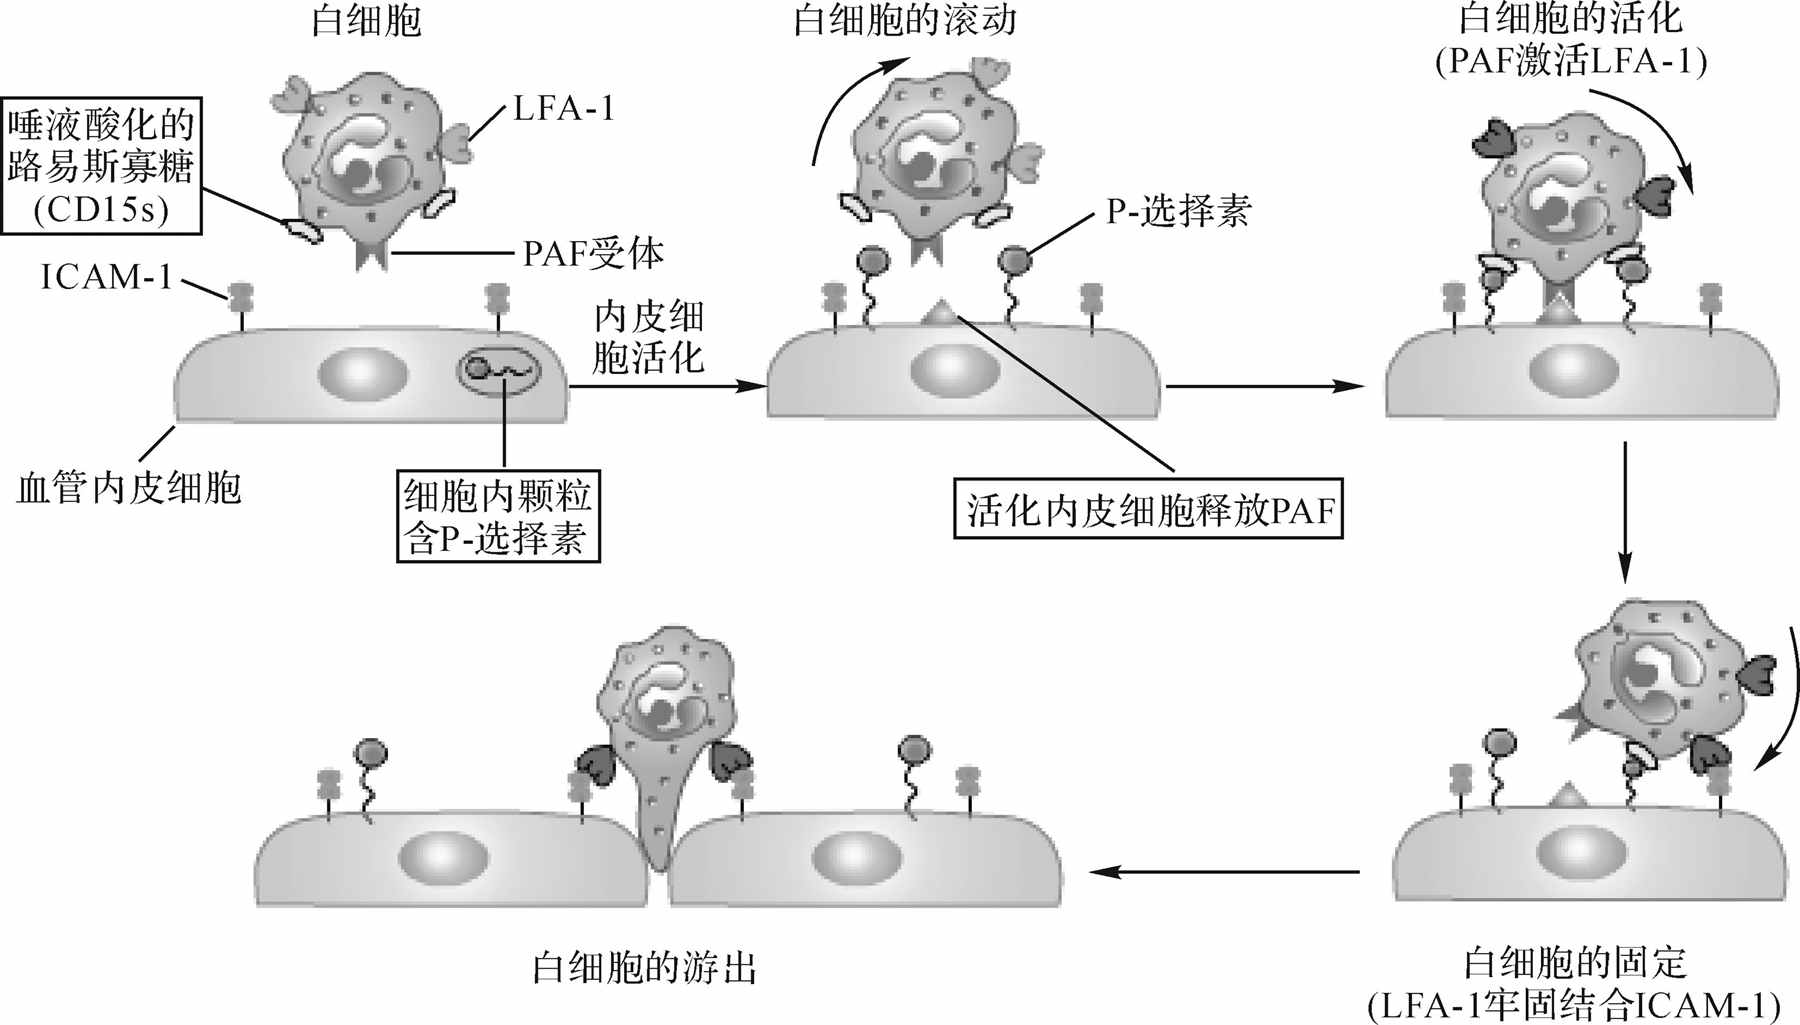
\includegraphics{./images/Image00120.jpg}
 \captionsetup{justification=centering}
 \caption{白细胞与血管内皮细胞黏附及渗出示意图}
 \label{fig8-10}
  \end{figure} 

(三)参与淋巴细胞归巢

淋巴细胞可借助黏附分子从血液回归至淋巴组织,此为淋巴细胞归巢(lymphocyte
homing)(图\ref{fig8-11})。介导淋巴细胞归巢的黏附分子称为淋巴细胞归巢受体(lymphocyte
homing
receptor,LHR),包括L-选择素、LFA-1、CD44等。LHR的配体称为地址素(addressin),主要表达于血管(尤其是淋巴结高内皮小静脉,HEV)内皮细胞表面,如外周淋巴结地址素(PNAd)、黏膜地址素细胞黏附分子(MadCAM-1)、ICAM-1、ICAM-2等。通过LFA-1/ICAM-1、L-选择素/PNAd、CD44/MadCAM-1等相互作用,介导淋巴细胞黏附并穿越HEV管壁回归至淋巴结中,继而再经淋巴管、胸导管进入血液,进行淋巴细胞再循环。

\begin{figure}[!htbp]
 \centering
 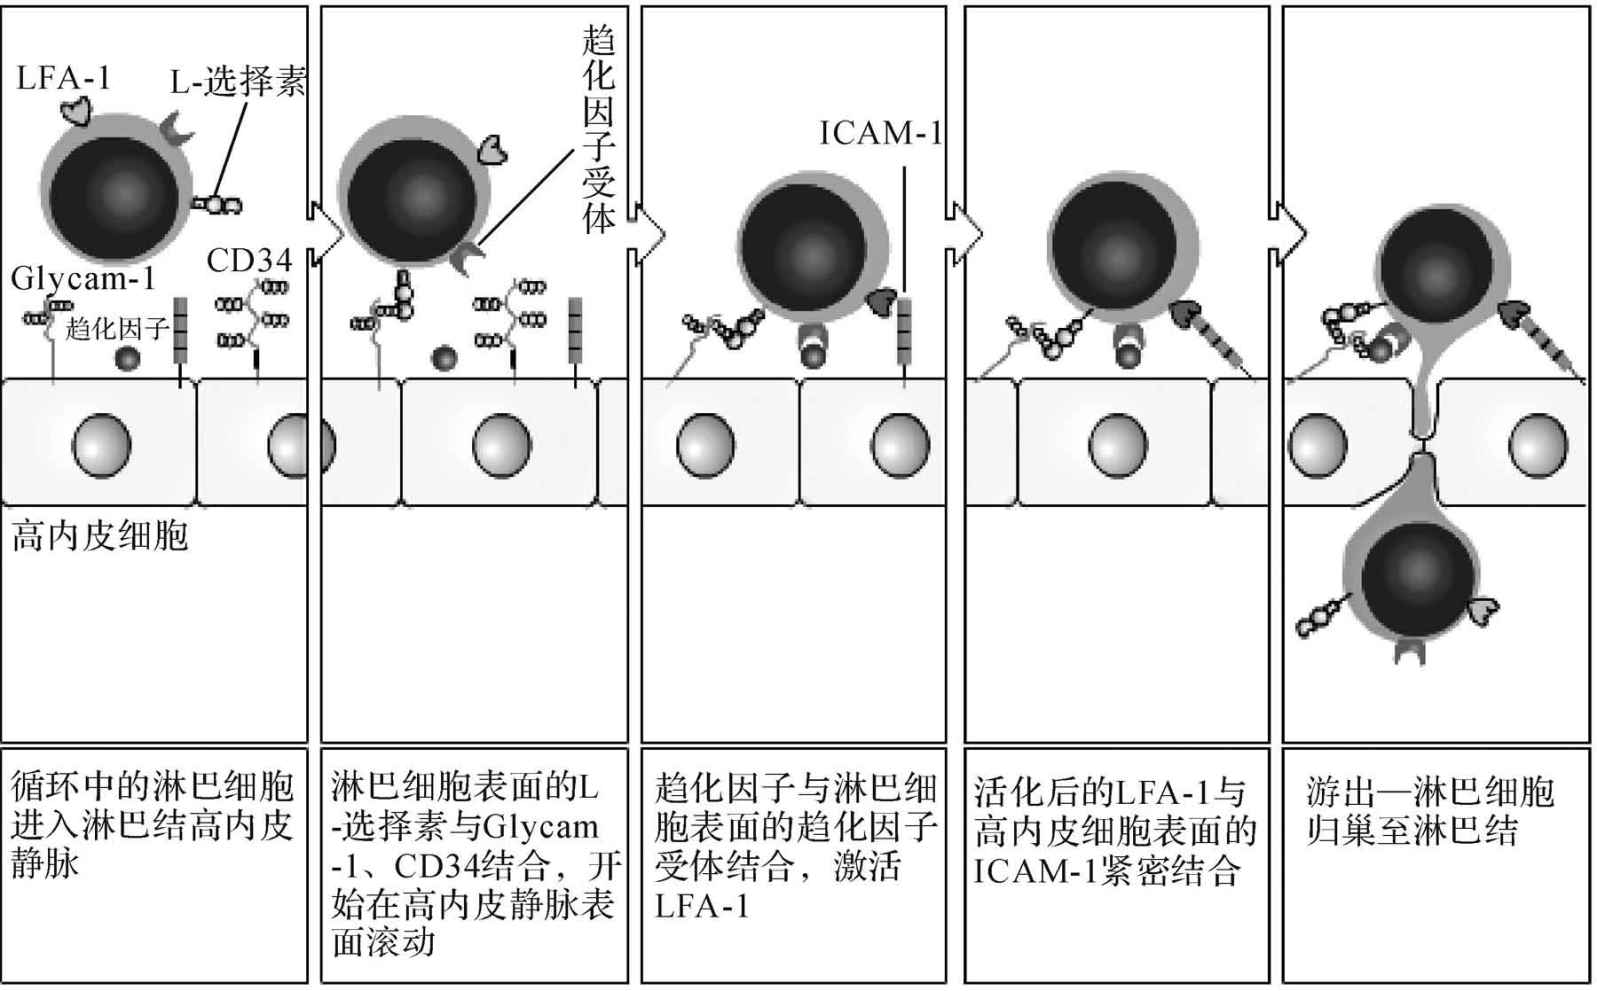
\includegraphics[width=.6\textwidth]{./images/Image00121.jpg}
 \captionsetup{justification=centering}
 \caption{参与淋巴细胞归巢}
 \label{fig8-11}
  \end{figure} 

(四)其他作用

IgSF等黏附分子参与诱导胸腺细胞分化与成熟;gpⅡb/Ⅲa、VNR-β3等整合素分子参与凝血及伤口修复过程;胚胎发育过程中,Cadherin等黏附分子参与细胞黏附及有序组合,对胚胎细胞发育形成组织和器官至关重要;黏附分子还参与细胞迁移和细胞凋亡的调节;等等。

\section{其他免疫细胞膜分子}


\subsection{促有丝分裂原受体}

\begin{figure}[!htbp]
 \centering
 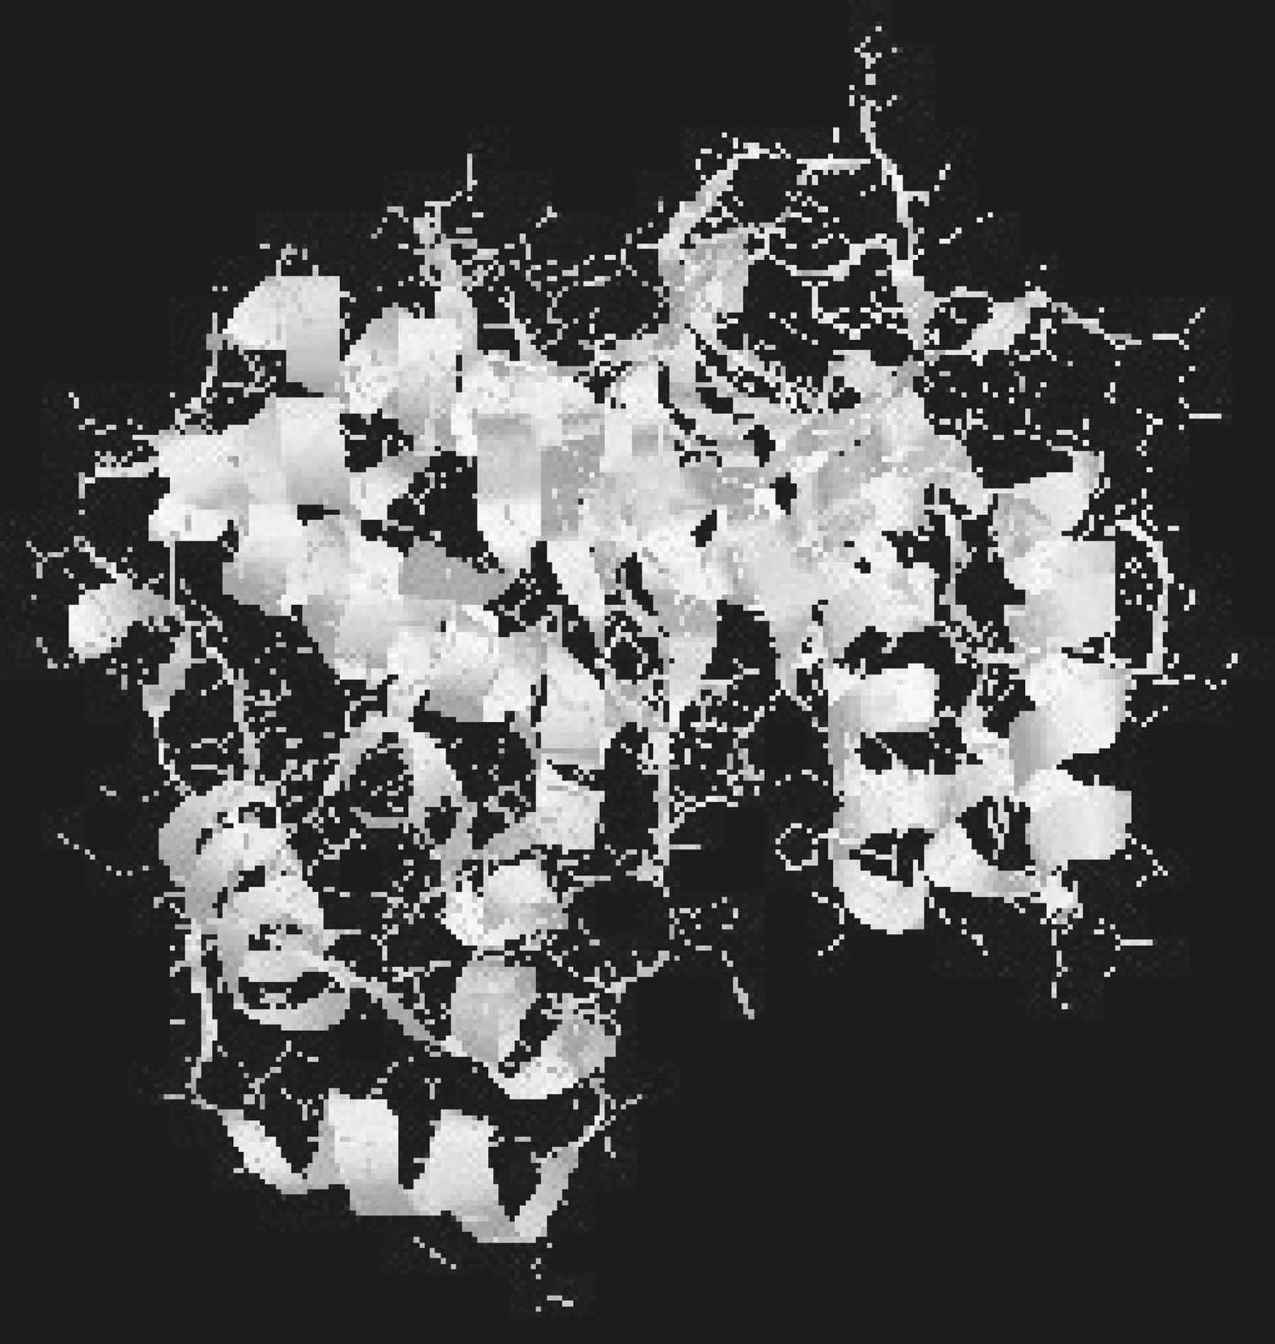
\includegraphics[width=.6\textwidth]{./images/Image00122.jpg}
 \captionsetup{justification=centering}
 \caption{促有丝分裂原受体}
 \label{fig8-12}
  \end{figure} 

有丝分裂原来自植物的糖蛋白或细菌产物,能与多种细胞膜糖类分子结合(受体)促进细胞活化、诱导分裂(图\ref{fig8-12})。

\begin{figure}[!htbp]
 \centering
 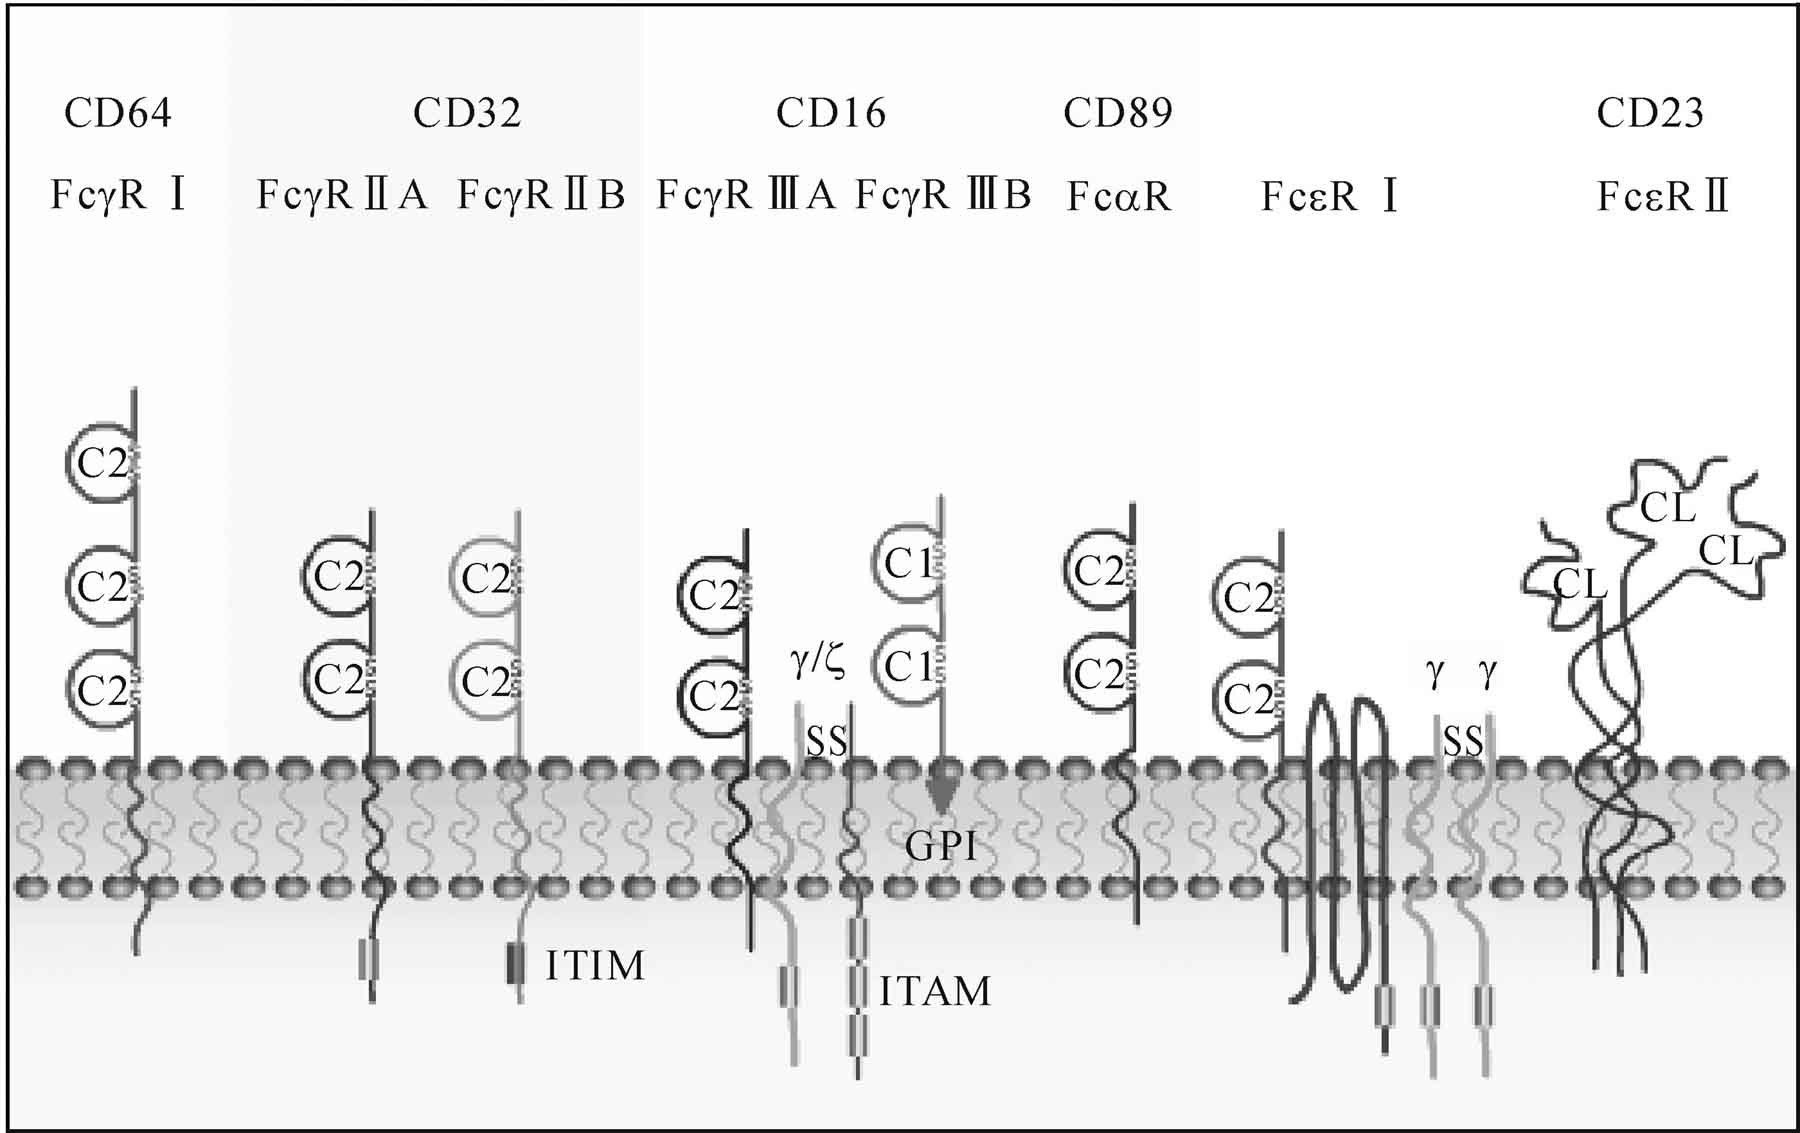
\includegraphics[width=.6\textwidth]{./images/Image00123.jpg}
 \captionsetup{justification=centering}
 \caption{各类Ig的Fc受体}
 \label{fig8-13}
  \end{figure} 


\subsection{IgFc受体}

体内多种细胞表面可表达IgFc受体,并通过二者结合,参与Ig
的功能。属于CD分子的Fc受体包括FcγR、FcαR和FcεR。其中FcγR分为FcγRⅠ、FcγRⅡ和FcγRⅢ三类;FcεR分为FcεRⅠ和FcεRⅡ两类,受体是糖蛋白,胞外都有Ig
样功能区,能与IgFc
结合(图\ref{fig8-13})。其功能为介导Ag识别,吞噬功能,Ag递呈,免疫细胞活化等。


\subsection{CK受体}

根据细胞因子受体cDNA序列以及受体胞膜外区氨基酸序列的同源性和结构征,可将细胞因子受体主要分为四种类型:免疫球蛋白超家族(IgSF)、造血细胞因子受体超家族、神经生长因子受体超家族和趋化因子受体。此外,还有些细胞因子受体的结构尚未完全搞清,如IL-10R、IL-12R等;有的细胞因子受体结构虽已搞清,但尚未归类,如IL-2Rα链(CD25)。免疫细胞表面表达多种CK受体,参与调节T、B细胞、单核吞噬细胞的生物学功能。

\begin{figure}[!htbp]
 \centering
 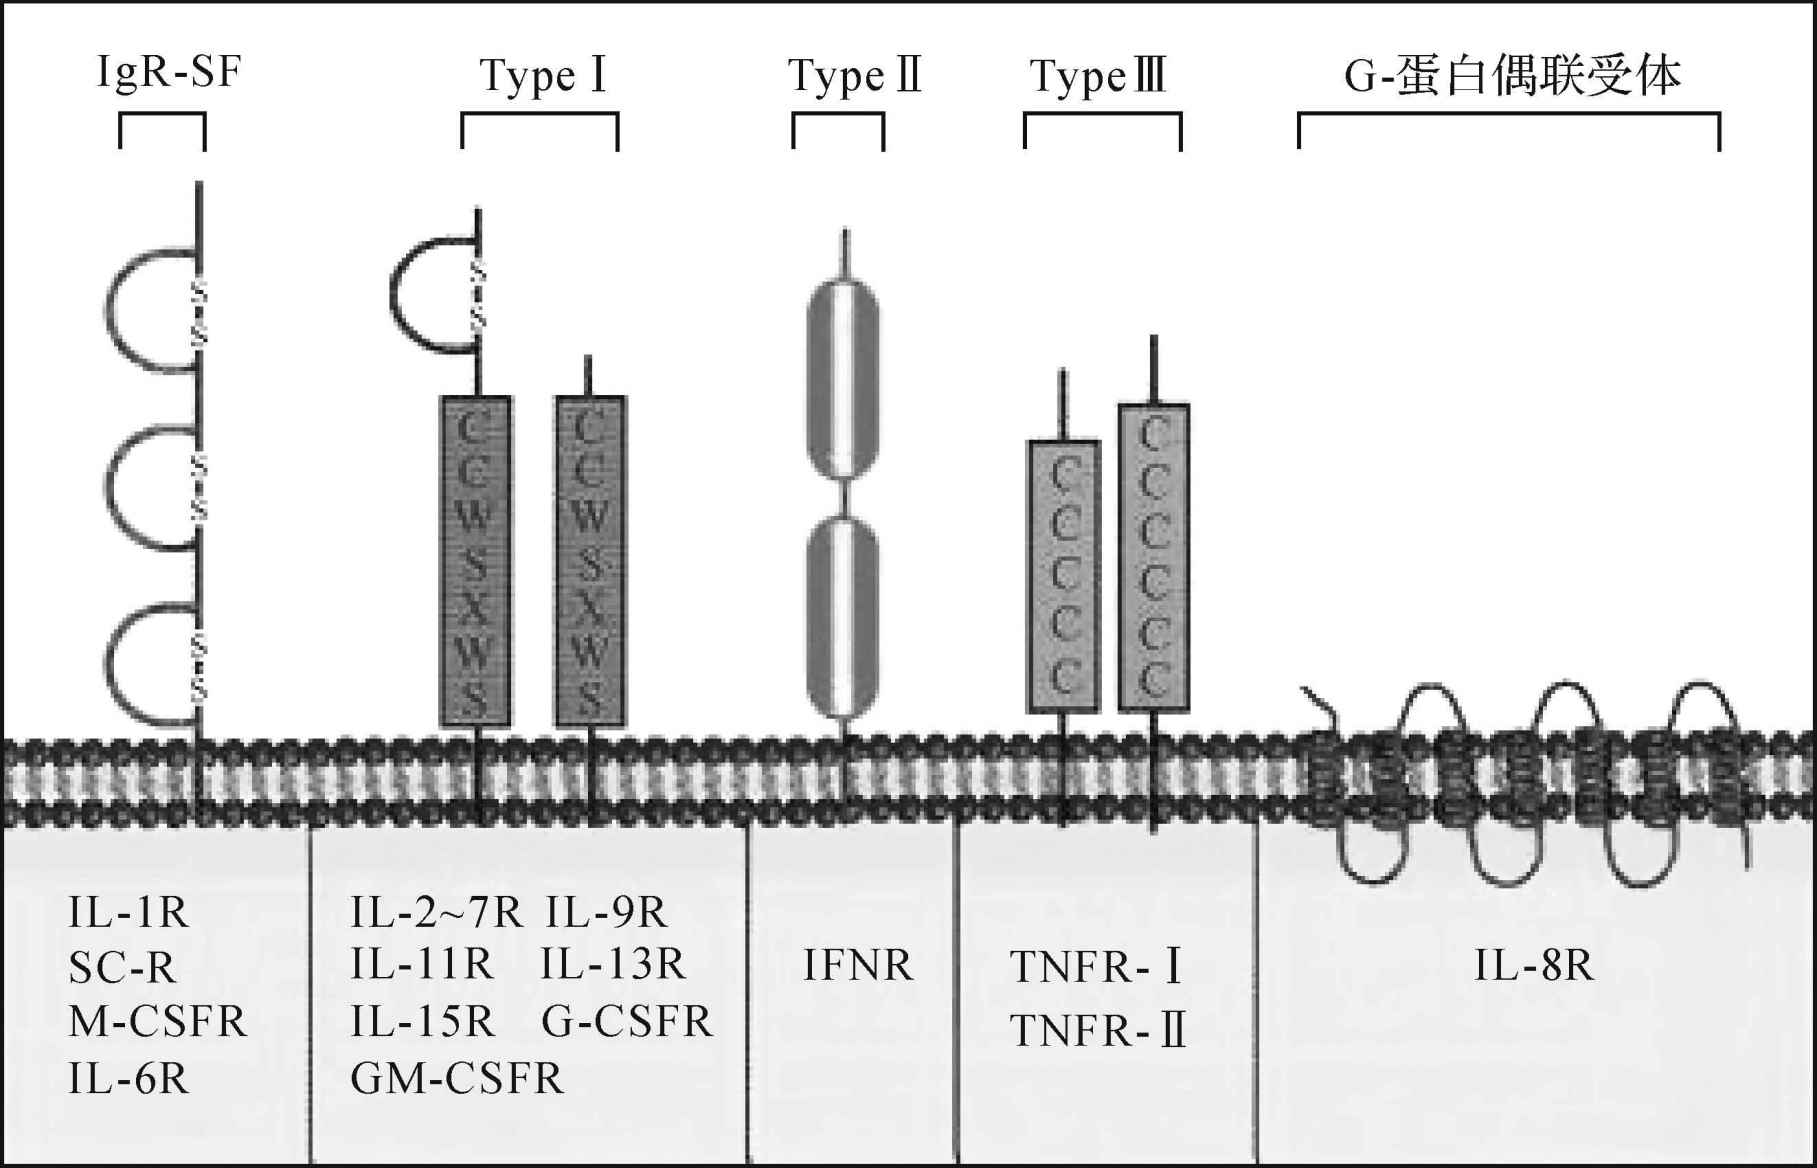
\includegraphics{./images/Image00124.jpg}
 \captionsetup{justification=centering}
 \caption{细胞因子受体超家族结构图}
 \label{fig8-14}
  \end{figure} 

细胞因子受体主要包括免疫球蛋白受体超家族(IgR---SF)、I型细胞因子受体家族、Ⅱ型细胞因子受体家族(干扰素受体家族)、Ⅲ型细胞因子受体家族(肿瘤坏死因子受体家族,TNFR---F)和七次跨膜受体家族(又称G---蛋白耦联受体家族),如图\ref{fig8-14}所示。


\subsection{补体受体}

中性粒细胞和单核-巨噬细胞高度表达补体受体,与吞噬功能有关(图\ref{fig8-15})。其配体为iC3b,但针对其他补体受体的单克隆抗体不能阻断CR4与iC3b的结合,证明CR4的存在。CR4与gp150/95为同一分子,对其功能尚有诸多不明之处。据认为CR4在排除组织内与iC3b结合的颗粒上起作用。它和CR3一样,与配体结合时需有二价离子的存在。

\begin{figure}[!htbp]
 \centering
 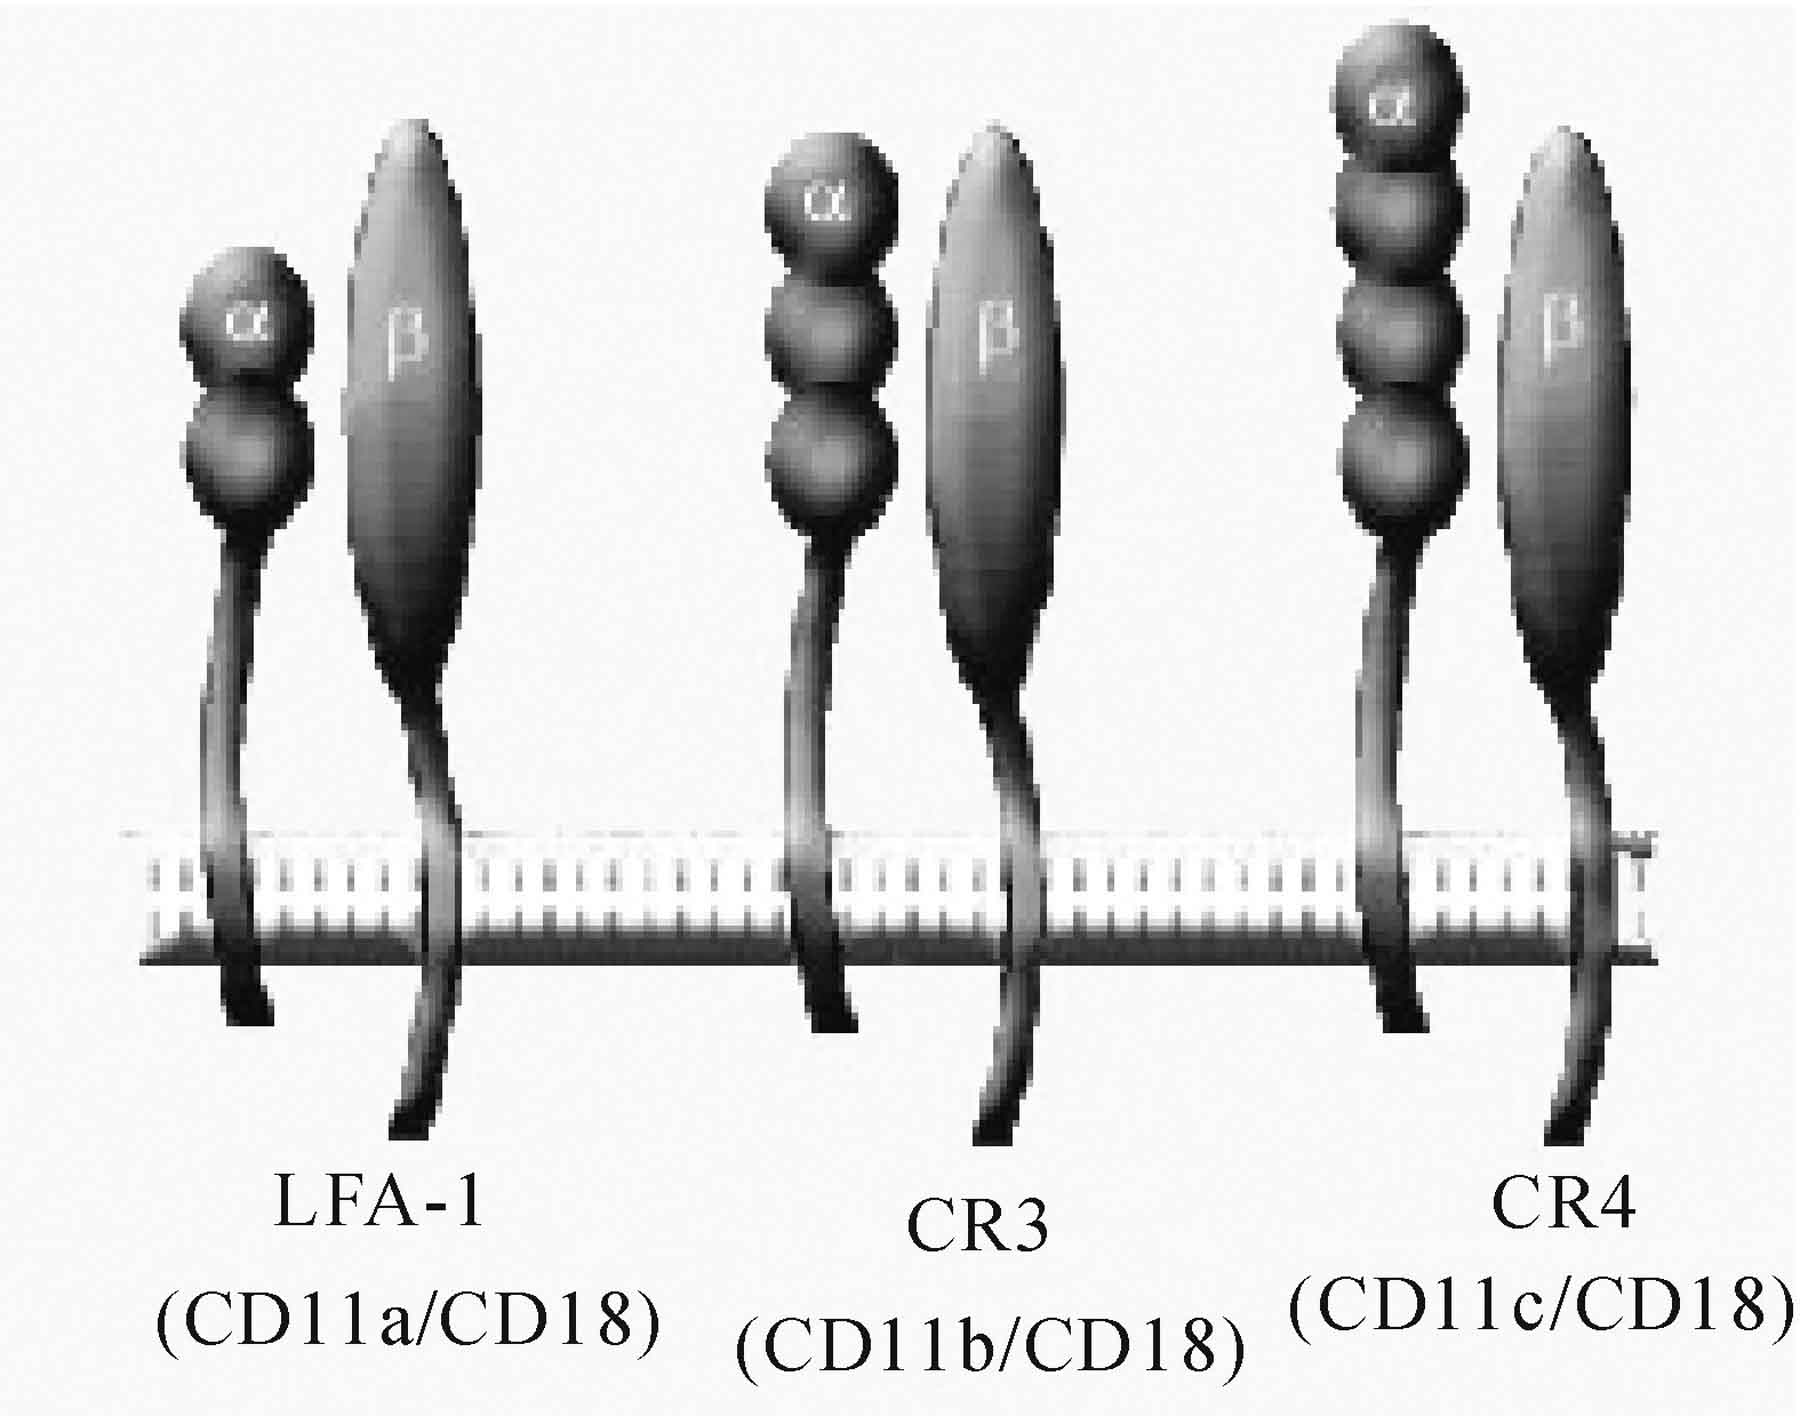
\includegraphics{./images/Image00125.jpg}
 \captionsetup{justification=centering}
 \caption{补体受体}
 \label{fig8-15}
  \end{figure} 


\subsection{内分泌激素、神经递质、神经肽受体}

免疫细胞表面可具有多种激素、神经递质和神经肽的受体,如雌激素、甲状腺素、肾上腺皮质激素、肾上腺素、前列腺素E、生长激素、胰岛素等激素的受体,内啡肽、脑啡肽、P物质等神经肽受体,组胺、乙酰胆碱、5-羟色胺、多巴胺等神经递质受体。免疫细胞表面的激素、神经肽和神经递质受体是机体神经内分泌免疫网络中的一个重要环节。

\noindent\textbf{【理解与思考】}

1.你能形象地解说机体免疫细胞膜分子的构成及其作用吗?

2.你就是一个免疫细胞,请从如何接受外界信号刺激,传递到内部产生作用作一表述。

3.当某一局部受到病原微生物的侵袭,请形象地描述淋巴细胞是如何到达病原微生物入侵部位的。

\noindent\textbf{【课外拓展】}

1.参与细胞凋亡的CD分子有哪些?

2.黏附分子与疾病有何关系?

3.黏附分子结合时,其结构有何变化?

4.参与T、B淋巴细胞抗原识别与活化的CD分子是如何互相影响的?

\noindent\textbf{【课程实验与研究】}

1.如何检测新出现的免疫细胞膜分子与其活性?

2.能够识别病原相关分子的模式识别受体是如何去鉴别的?

3.免疫负相调控机制与CD分子有何关联?

\noindent\textbf{【课程研讨】}

1.阐述某一种白细胞分化抗原的研究进展。

2.免疫细胞膜缺失会导致什么样的结果?

3.黏附分子与肿瘤的发生有何关联?

4.目前,黏附分子的研究热点是什么?你认为将来的研究方向是什么?要解决什么难题?

5.免疫识别的结构基础与相关机制研究能解决什么问题?

\noindent\textbf{【课后思考】}

1.CD分子、黏附分子的概念。

2.简述与T细胞识别、黏附及活化有关的主要CD分子与其作用。

3.简述与B细胞识别、黏附及活化有关的主要CD分子与其作用。

\noindent\textbf{【课外阅读】}

\begin{center}
 \textbf{\Large CD45在淋巴细胞活化中的研究}
 \end{center}

CD45又称为白细胞共同抗原(LCA),是一种单链跨膜糖蛋白,是蛋白酪氨酸磷酸酶(PTPase)家族成员,它广泛地存在于造血系细胞,如T细胞、B细胞、自然杀伤细胞和巨噬细胞表面。CD45通过对蛋白酪氨酸激酶(PTKs)的调节,在淋巴细胞的发育和活化中起重要作用。

CD45至少有9个变构体(如CD45RA、CD45RB、CD45RC、CD45RO等),由4~6个外显子(常见的有A、B、C等)交替剪接而成。这些变构体的胞外结构不同,但有共同的胞浆结构。单个淋巴细胞可同时表达多个变构体。CD45变构体在T细胞和B细胞上的表达有所不同,在T细胞各功能亚群上以及在T细胞发育和活化的各阶段也存在不同。

\begin{center}
 {\large 一、CD45对Src家族蛋白酪氨酸激酶的调节作用}
 \end{center}

PTKs是淋巴细胞活化信号传递过程中的重要介质,主要包括3个家族:Src家族、Syr家族和Jak家族。CD45通过对Src家族PTKs的调节而在淋巴细胞活化中起重要作用。其分子结构上有两个关键的调节性酪氨酸磷酸化位点,一个位于激酶结构域,另一个位于C末端尾,前者的磷酸化可增强激酶的活性,称为活化位点;后者的磷酸化则抑制激酶活性,称为抑制位点。

CD45可以同时使活化位点和抑制位点去磷酸化从而控制Src激酶的活性,因此CD45同时具备阴性调节和阳性调节作用。在静止细胞,CD45可以和磷酸根竞争抑制位点同时使活化性位点去磷酸化,其综合效应是使Src激酶处于非活化状态。当受体和抗原结合后,膜蛋白的位置发生改变,Src激酶向抗原受体方向位移,从而使Src激酶和CD45分离,活化位点磷酸化而使Src激酶活化,此时CD45是阳性调节。在整合素介导的细胞黏附过程中,Src激酶和CD45同时向黏附位点位移,此时CD45仍使活化位点去磷酸化,从而发挥阴性调节作用。

\begin{center}
 {\large 二、CD45对抗原-受体信号的调节作用}
 \end{center}

TCR复合体包括一个异二聚体(TCRαβ或TCRγδ)、CD3复合体和一个ζ链同二聚体。同样,BCR复合体也包含多个亚单位。无论是TCR或BCR,其信号传导均以PTKs的活化而开始。

研究显示,缺乏CD45的细胞接受抗原刺激后,不能产生有效的活化信号。通过分析发现,这种抗原-受体信号的传导异常是由于缺乏Src激酶的调节而引起的,缺乏CD45的T细胞,Src激酶抑制性位点的磷酸化程度增高,故不能形成有效的信号传导,说明CD45在淋巴细胞的抗原-受体信号传导中起着关键作用。

\begin{center}
 {\large 三、CD45在调节细胞黏附中的作用}
 \end{center}

抗原被抗原特异性受体识别以及T细胞和抗原递呈细胞之间的黏附是T细胞活化的两个同等重要的过程。由于TCR与抗原的亲合力较低,需要其他的蛋白质(如整合素)来稳定细胞间的接触才能有效地使T细胞活化。当整合素和配体结合后,Src家族激酶和CD45分子均向黏附位点移位,Src家族激酶由于其高度亲和力的结合位点与黏附分子上的黏附位点结合而活化,此时尽管CD45仍使抑制位点去磷酸化,但其作用是次要的,不足以抑制激酶的活化,可见CD45对细胞间的黏附起阴性调节作用。

\begin{center}
 {\large 四、CD45胞外结构在信号传导中的作用}
 \end{center}

Robert等研究发现,在缺乏CD45跨膜和胞外结构的情况下,CD45的胞内结构仍可以参与TCR的信号传导,提示CD45胞内结构的酶活性对TCR的信号传导是必要和充分的。那么,CD45的胞外结构在信号传导中起什么作用呢?研究表明,某些CD45变构体的表达与淋巴细胞的成熟及活化存在密切联系,从而提示不同的CD45变构体可能与T细胞的功能有关。向CD45阴性细胞内转染不同的CD45变构体cDNA,发现对TCR的信号传导的影响也不同。说明不同的变构体对T细胞活化的调节不同。Dianzani等认为,这可能是由于不同的变构体与细胞表面上不同分子选择性结合的结果。也就是说,CD45的胞外部分可能提供信号传导的特异性,胞内部分参与信号的传导。

\begin{center}
 {\large 五、CD45分子在淋巴细胞发育中的作用}
 \end{center}

CD45分子可能对T细胞在胸腺内的选择和发育起着非常重要的作用。Deans等研究发现,CD45RA阳性的胸腺细胞可以分化为T细胞,而CD45RO阳性的胸腺细胞则在胸腺内被清除。早期的研究显示,CD4\textsuperscript{+}
CD45RA\textsuperscript{+} T细胞是抑制-诱导亚群,而CD4\textsuperscript{+}
CD45RA\textsuperscript{-}
T细胞是辅助-诱导亚群。然而事实远比这复杂得多,因为有研究显示,活化T细胞仍保留CD45RA\textsuperscript{+}
,而且CD45RA\textsuperscript{-} 和CD45RA\textsuperscript{+}
T细胞之间也可以相互转换。

敲除小鼠CD45基因后,发现其胸腺细胞的发育被严重阻断,从而使CD4\textsuperscript{-}
CD8\textsuperscript{-} 胸腺细胞增多,CD4\textsuperscript{+}
CD8\textsuperscript{+}
胸腺细胞减少,结果外周T细胞急剧减少,T细胞TCR对抗原刺激无反应,也不能产生细胞毒性反应。此时B细胞的数量虽然正常,但外周未成熟细胞明显增多。可见,CD45对T细胞和B细胞的发育和功能都非常重要。

\begin{center}
 {\large 六、CD45调节淋巴细胞的活性}
 \end{center}

研究显示,缺乏CD45的CD4\textsuperscript{+} 、CD8\textsuperscript{+}
T细胞,其抗原特异性增殖能力、分泌IFN-γ能力以及溶解靶细胞能力均降低。如果使CD4\textsuperscript{+}
、CD8\textsuperscript{+}
T细胞重新表达CD45,则可恢复这些能力。但Irie-Sasaki等的研究发现,CD45对细胞因子受体介导的信号传导起阴性调节作用,并且发现破坏CD45基因则可以增强细胞因子和IFN-γ受体介导的细胞活化。

淋巴细胞活化是一个复杂过程,包括PTKs的活化、某些细胞蛋白酪氨酸的磷酸化、细胞内Ca\textsuperscript{2+}
浓度的增加、磷酸肌醇的水解、蛋白激酶C和Ras的活化等。缺乏CD45分子的淋巴细胞在TCR受体抗原刺激后,酪氨酸激酶活性降低,磷酸肌醇及细胞内Ca\textsuperscript{2+}
代谢也降低,因而不能有效地传导活化信号。如通过转基因技术使T细胞重新表达CD45分子,则可恢复TCR的信号传导能力,说明CD45分子在TCR的信号传导中是非常重要的。

\begin{center}
 {\large 七、CD45结合蛋白的作用}
 \end{center}

CD45结合蛋白(CD45AP)又称为淋巴细胞磷酸酶结合蛋白(LPAP),是一个包含有198个氨基酸的蛋白质。CD45AP主要表达在T细胞和B细胞表面,CD45AP的表达与CD45的表达密切相关。在CD45阴性细胞,细胞表面检测不到CD45AP的表达,而CD45AP
mRNA仍有表达。研究发现,此时CD45AP仍有合成,但合成后很快降解。用CD45cDNA转染CD45阴性细胞,结果可以恢复CD45AP的表达,提示CD45AP和CD45结合可防止其降解。CD45AP的功能尚不清楚,鉴于CD45AP的表达受CD45的严格调节,所以认为CD45AP在CD45介导的淋巴细胞信号传导中发挥重要作用。但也有学者发现,缺乏CD45AP的小鼠,其胸腺细胞及脾细胞的分化发育是正常的,而且这些细胞的P56\textsuperscript{Lck}
的活性与正常细胞没有区别,因而认为CD45AP在CD45对Src激酶活性的调节过程中并不是必需的。

CD45是一个重要的跨膜分子,它以其蛋白酪氨酸磷酸酶活性使蛋白酪氨酸激酶的抑制位点的酪氨酸去磷酸化从而使其活化,进而在T细胞活化的信号传递中起重要作用。近年来,随着对CD45认识的不断深入,人们试图利用单克隆抗体或药物阻断CD45介导的信号传导来阻断淋巴细胞的活化,进而应用于诱导免疫耐受和逆转移植排斥反应的研究,并取得了较好的效果。但CD45及其结合蛋白在淋巴细胞的发育、增殖和活化过程中的确切作用机制仍不甚清楚,CD45及其阻断措施在调节淋巴细胞活化中的作用,特别是在诱导免疫耐受及逆转排斥反应中的应用还需要进一步研究。

\begin{center}
 \textbf{\Large 改造T细胞受体限制HIV扩散}
 \end{center}

通过基因改革工程,研究人员让“杀手”T细胞更好地限制了HIV在培养液中的扩散。他们在日前在线出版的《自然---医学》期刊中说,这种能力升高的T细胞还能识别已经发生变异并试图逃过免疫反应的病毒。

T细胞受体(TCR)能够识别病毒蛋白质碎片,并在受感染细胞表面发出警告信息,T细胞因此得知了HIV的出现。目前,分离这种能够识别HIV的特别T细胞的方法主要基于克隆取自HIV患者的细胞,这是一个缓慢而费力的过程,而且,这些细胞中的TCR鉴别受感染细胞的能力很弱。病毒能够通过变异而逃脱探测。

James
Riley和同事利用噬菌体表面展示技术,从取自HIV患者的T细胞分离出TCR,这种TCR能很好地鉴别出HIV的存在。然后,他们通过基因工程改造这种TCR,让它能更好地探寻病毒。将这种TCR置入T细胞中,结果产生出力量更大的“杀手”细胞,能够在培养液中更好地限制HIV的扩散。

(资料来源:Nature Medicine,doi:10.1038/nm.1779,Bent K
Jakobsen,James L Riley)

